\documentclass[Royal,times,sageh]{sagej}
%DIF LATEXDIFF DIFFERENCE FILE
%DIF DEL Manuscript-Data-Package2.tex                Sat May 31 12:56:15 2025
%DIF ADD Manuscript-Data-Package-1Round-Review.tex   Sat May 31 20:02:28 2025

\usepackage{moreverb,url,natbib, multirow, tabularx}
\usepackage[colorlinks,bookmarksopen,bookmarksnumbered,citecolor=red,urlcolor=red]{hyperref}



% tightlist command for lists without linebreak
\providecommand{\tightlist}{%
  \setlength{\itemsep}{0pt}\setlength{\parskip}{0pt}}

%DIF 12-22d12
%DIF < % From pandoc table feature
%DIF < \usepackage{longtable,booktabs,array}
%DIF < \usepackage{calc} % for calculating minipage widths
%DIF < % Correct order of tables after \paragraph or \subparagraph
%DIF < \usepackage{etoolbox}
%DIF < \makeatletter
%DIF < \patchcmd\longtable{\par}{\if@noskipsec\mbox{}\fi\par}{}{}
%DIF < \makeatother
%DIF < % Allow footnotes in longtable head/foot
%DIF < \IfFileExists{footnotehyper.sty}{\usepackage{footnotehyper}}{\usepackage{footnote}}
%DIF < \makesavenoteenv{longtable}
%DIF -------


\usepackage{booktabs}
\usepackage{longtable}
\usepackage{array}
\usepackage{multirow}
\usepackage{wrapfig}
\usepackage{float}
\usepackage{colortbl}
\usepackage{pdflscape}
\usepackage{tabu}
\usepackage{threeparttable}
\usepackage{threeparttablex}
\usepackage[normalem]{ulem}
\usepackage{makecell}
\usepackage{xcolor}
%DIF PREAMBLE EXTENSION ADDED BY LATEXDIFF
%DIF UNDERLINE PREAMBLE %DIF PREAMBLE
\RequirePackage[normalem]{ulem} %DIF PREAMBLE
\RequirePackage{color}\definecolor{RED}{rgb}{1,0,0}\definecolor{BLUE}{rgb}{0,0,1} %DIF PREAMBLE
\providecommand{\DIFaddtex}[1]{{\protect\color{blue}\uwave{#1}}} %DIF PREAMBLE
\providecommand{\DIFdeltex}[1]{{\protect\color{red}\sout{#1}}} %DIF PREAMBLE
%DIF SAFE PREAMBLE %DIF PREAMBLE
\providecommand{\DIFaddbegin}{} %DIF PREAMBLE
\providecommand{\DIFaddend}{} %DIF PREAMBLE
\providecommand{\DIFdelbegin}{} %DIF PREAMBLE
\providecommand{\DIFdelend}{} %DIF PREAMBLE
\providecommand{\DIFmodbegin}{} %DIF PREAMBLE
\providecommand{\DIFmodend}{} %DIF PREAMBLE
%DIF FLOATSAFE PREAMBLE %DIF PREAMBLE
\providecommand{\DIFaddFL}[1]{\DIFadd{#1}} %DIF PREAMBLE
\providecommand{\DIFdelFL}[1]{\DIFdel{#1}} %DIF PREAMBLE
\providecommand{\DIFaddbeginFL}{} %DIF PREAMBLE
\providecommand{\DIFaddendFL}{} %DIF PREAMBLE
\providecommand{\DIFdelbeginFL}{} %DIF PREAMBLE
\providecommand{\DIFdelendFL}{} %DIF PREAMBLE
%DIF HYPERREF PREAMBLE %DIF PREAMBLE
\providecommand{\DIFadd}[1]{\texorpdfstring{\DIFaddtex{#1}}{#1}} %DIF PREAMBLE
\providecommand{\DIFdel}[1]{\texorpdfstring{\DIFdeltex{#1}}{}} %DIF PREAMBLE
%DIF COLORLISTINGS PREAMBLE %DIF PREAMBLE
\RequirePackage{listings} %DIF PREAMBLE
\RequirePackage{color} %DIF PREAMBLE
\lstdefinelanguage{DIFcode}{ %DIF PREAMBLE
%DIF DIFCODE_UNDERLINE %DIF PREAMBLE
  moredelim=[il][\color{red}\sout]{\%DIF\ <\ }, %DIF PREAMBLE
  moredelim=[il][\color{blue}\uwave]{\%DIF\ >\ } %DIF PREAMBLE
} %DIF PREAMBLE
\lstdefinestyle{DIFverbatimstyle}{ %DIF PREAMBLE
	language=DIFcode, %DIF PREAMBLE
	basicstyle=\ttfamily, %DIF PREAMBLE
	columns=fullflexible, %DIF PREAMBLE
	keepspaces=true %DIF PREAMBLE
} %DIF PREAMBLE
\lstnewenvironment{DIFverbatim}{\lstset{style=DIFverbatimstyle}}{} %DIF PREAMBLE
\lstnewenvironment{DIFverbatim*}{\lstset{style=DIFverbatimstyle,showspaces=true}}{} %DIF PREAMBLE
\lstset{extendedchars=\true,inputencoding=utf8}

%DIF END PREAMBLE EXTENSION ADDED BY LATEXDIFF

\begin{document}


\setcitestyle{aysep={,}}

\title{ActiveCA: Time Use Data from the General Social Survey of Canada
to Study Active Travel}

\runninghead{}

\author{Anon1\affilnum{}, Anon2\affilnum{}, Anon3\affilnum{}}

\affiliation{\affilnum{}{}}



\begin{abstract}
This paper describes \{ActiveCA\}, an open data product with Canadian
time use data. \{ActiveCA\} is an R data package that contains
analysis-ready data related to active travel spanning almost 40 years,
extracted from cycles 2 (1986), 7 (1992), 12 (1998), 19 (2005), 24
(2010), \DIFdelbegin \DIFdel{and }\DIFdelend 29 (2015)\DIFdelbegin \DIFdel{of Canada's }\DIFdelend \DIFaddbegin \DIFadd{, and 34 (2022) of the Time Use Survey (TUS) cicles
from the }\DIFaddend General Social Survey \DIFaddbegin \DIFadd{(GSS)}\DIFaddend . Active travel is characterized by
mode, with walking being part of every cycle and bicycling starting in
1992. The attributes of active trips are the types of locations of
origins and destinations, the duration of trips, and episode weights for
expanding the trips to population-wide estimates. Based on the year of
the survey, a variety of locations are coded. In earlier cycles, these
include home, work or school, and other's home, whereas in later cycles
these are augmented with locations such as grocery stores, restaurants,
outdoor destinations, and others. The geographical resolution includes
the province and whether the episode was in an urban or rural setting.
\end{abstract}

\keywords{Active; mobility; walking; cycling; travel time; time-use;
General Social Survey}

\maketitle

\section{Introduction}\label{introduction}

The objective of this paper is to introduce \{ActiveCA\}, an open data
product with \DIFdelbegin \DIFdel{time use data from Canada's }\DIFdelend \DIFaddbegin \DIFadd{data from all Time Use Survey (TUS) cycles of the }\DIFaddend General
Social Surveys \DIFaddbegin \DIFadd{(GSSs)}\DIFaddend . Open data products (ODPs) are the outcome of a
process that transforms raw data (open or not) into analysis-ready data,
following a transparent process in which all stages of development
follow open principles \citep{arribas-bel2021}. ODPs, while still open,
differ from general open data in their degree of ease of access, their
heightened usability, and potentially the value they add to the raw
data.

\{ActiveCA\} provides analysis-ready data concerning active travel in
Canada spanning a period of almost 40 years\DIFdelbegin \DIFdel{. The source of these data is
Canada's program of General Social Surveys (GSSs). This program }\DIFdelend \DIFaddbegin \DIFadd{, obtained from the TUS
cycles of the Canadian GSS. The GSS program }\DIFaddend is designed to provide
cross-sectional data on topics of interest to improve the well-being of
Canadians. As part of this program, every five to seven years the survey
is done on the topic of time use \DIFaddbegin \DIFadd{(TUS)}\DIFaddend . Concretely, \{ActiveCA\} covers
Cycles 2 (1986), 7 (1992), 12 (1998), 19 (2005), 24 (2010), \DIFdelbegin \DIFdel{and }\DIFdelend 29 (2015)\DIFdelbegin \DIFdel{of the GSS}\DIFdelend \DIFaddbegin \DIFadd{,
and 34 (2022) of the TUS}\DIFaddend . Time use data in these surveys is coded using
a very fine grain, from time spent in chores, leisure, and sleeping, to
time spent working or at school. These surveys have proved valuable in
investigations of mobility and quality of life
\citep{spinneyTransport2009}, the relationship between active travel and
transit use \citep{lachapelleLonger2016}, and travel behavior and time
poverty \citep{kimFacing2024}, to name but a few examples.

\DIFdelbegin \DIFdel{For \{ActiveCA\} and using GSS }\DIFdelend \DIFaddbegin \DIFadd{Using }\DIFaddend Public Use Microdata Files (PUMFs) \DIFaddbegin \DIFadd{from the Time Use Survey (TUS)}\DIFaddend ,
we extracted all data \DIFdelbegin \DIFdel{needed }\DIFdelend \DIFaddbegin \DIFadd{necessary }\DIFaddend to characterize active travel in Canada
\DIFdelbegin \DIFdel{,
namely, episodes where the activity was identified as }\DIFdelend \DIFaddbegin \DIFadd{- specifically, episodes in which the activity involved }\DIFaddend moving between
an origin and a destination \DIFdelbegin \DIFdel{, either }\DIFdelend by walking or cycling. Although Statistics
Canada \DIFdelbegin \DIFdel{offers Public Use Microdata Files and }\DIFdelend \DIFaddbegin \DIFadd{provides PUMFs and accompanying }\DIFaddend documentation for the GSS program
\citep[see][]{statisticscanada2024}, accessing \DIFdelbegin \DIFdel{these
files, and preparing them }\DIFdelend \DIFaddbegin \DIFadd{and preparing these files
}\DIFaddend for analysis is not a straightforward \DIFdelbegin \DIFdel{matter,
given }\DIFdelend \DIFaddbegin \DIFadd{task due to }\DIFaddend their size and
complexity. The process of extracting information of interest from the
source files is time-consuming, tedious, and challenging and/or prone to
error due to the expertise required to work with these files. To create
\{ActiveCA\} we \DIFdelbegin \DIFdel{collected, cleaned}\DIFdelend \DIFaddbegin \DIFadd{selected, labelled}\DIFaddend , and processed the \DIFdelbegin \DIFdel{cycles of the GSS surveys concerning time use }\DIFdelend \DIFaddbegin \DIFadd{TUS cycles }\DIFaddend to make
them ready for analysis.

\{ActiveCA\} is distributed as an \DIFdelbegin \DIFdel{R }\DIFdelend \DIFaddbegin \texttt{\DIFadd{R}} \DIFaddend package with a number of
data objects and their documentation. \DIFdelbegin \DIFdel{R }\DIFdelend \DIFaddbegin \texttt{\DIFadd{R}} \DIFaddend packages contain code,
data, and documentation in a standardized format that can be installed
by R users via a software repository, such as CRAN (Comprehensive R
Archive Network) or GitHub, which makes them an adroit medium to
distribute analysis-ready data.

Given the level of interest in active travel
\citep[e.g.,][]{mccurdySupport2023}, reducing the barriers to using data
contained in rich, but difficult to access and use surveys, such as \DIFdelbegin \DIFdel{Canada's GSSs}\DIFdelend \DIFaddbegin \DIFadd{TUS}\DIFaddend ,
is a worthy endeavour that can only improve data-driven decisions in
transportation, urban, and health policy.

The rest of this paper discusses the sources of data, and the process
implemented to retrieve and package them. Then, we explain how to use
the package and show some selected examples of analysis to whet the
imagination of potential users. This ODP provides not only data that are
easy to use, but also all the code and documentation that make this a
reproducible research project. In summary, \{ActiveCA\} aims to
implement and inspire the best principles of open spatial sciences
\citep{paez_open_2021, brunsdon_opening_2021}.

\section{\DIFdelbegin \DIFdel{General Social }\DIFdelend \DIFaddbegin \DIFadd{The Time Use }\DIFaddend Survey (\DIFdelbegin \DIFdel{GSS}\DIFdelend \DIFaddbegin \DIFadd{TUS}\DIFaddend )
collection}\DIFdelbegin %DIFDELCMD < \label{general-social-survey-gss-collection}
%DIFDELCMD < %%%
\DIFdelend \DIFaddbegin \label{the-time-use-survey-tus-collection}
\DIFaddend 

Statistics Canada \citeyearpar{statisticscanada2024} conducts GSS
surveys to obtain data on social trends to track changes in Canadians'
living conditions and well-being over time. The series of survey on time
use are used to understand how Canadian residents spend and manage their
time, and what factors contribute to their happiness and stress. The GSS
program was created in 1985, and is serialized to provide a collection
of annual, representative cross-sectional surveys.

The topics of the survey cycle every few years to cover topics that
include family, health, social identity, and every five to seven years
time use. The first Canadian \DIFdelbegin \DIFdel{time use survey }\DIFdelend \DIFaddbegin \DIFadd{TUS }\DIFaddend done as part of the GSS program was
conducted in 1986, and the most recent was completed in \DIFdelbegin \DIFdel{2015. }\DIFdelend \DIFaddbegin \DIFadd{2022. }\DIFaddend These Time
Use Surveys \citep{statisticscanada2022} collect data on respondents'
participation and time spent on a wide range of everyday activities
using a 24-hour retrospective diary, with information on the location of
these activities (e.g.~at home, at work, etc.) and, for non-personal
activities, the people who were present with the respondent at the time
of the activity. In addition, time-use surveys also cover topics related
to leisure time, work-life balance, health, commuting, culture and
sports, and many others.

\DIFaddbegin \DIFadd{TUS allows researchers to identify the origin and destination of trips,
travel times and modes of transport used, providing a valuable dataset
for analyzing active travel behavior. It also provides the empirical
basis for tools used in transportation analysis, such as the development
of impedance functions for accessibility analysis, a measure of the ease
with which people can reach destinations and opportunities
\mbox{%DIFAUXCMD
\citep{hansen1959}}\hskip0pt%DIFAUXCMD
. The Canadian TUS is unique at the national level in
collecting detailed information on travel behaviour. Its consistent
application across survey cycles enables the identification of long-term
trends, with some questions present in the questionnaires since the
first application of the survey.
}

\DIFadd{Most respondents to the 2022 TUS completed it online, reflecting
Statistics Canada's effort to adapt to technological changes and growing
time demands by offering greater flexibility and convenience
\mbox{%DIFAUXCMD
\citep{statisticscanada2022}}\hskip0pt%DIFAUXCMD
. While such methodological changes may
affect data comparability over time, it is not possible to determine
whether observed differences result from actual population changes or
shifts in data collection methods. Despite rigorous efforts to ensure
data quality, the use of electronic questionnaires may have influenced
estimates. Statistics Canada assessed the impact of collection mode on a
limited set of key questions, constrained by sample size. Importantly,
none of the variables used in this research are }\texttt{\DIFadd{R}} \DIFadd{package in
the 2022 PUMF User Guide as unsuitable for trend analysis.
}

\DIFadd{Until 2022, Statistics Canada employed a telephone-based sampling frame,
which was replaced by a dwelling-based frame in the most recent cycle.
Each survey cycle spans a 12-month period, typically from July to the
following July. The target population includes all Canadians aged 15 and
over, excluding residents of the Yukon, Northwest Territories, and
Nunavut, full-time institutional residents, and individuals living on
Indigenous reserves.
}

\DIFadd{The survey encompasses both rural and urban areas, including
metropolitan and non-metropolitan regions, to ensure a diverse and
representative sample. For sampling, the ten provinces were divided into
geographic strata. Several Census Metropolitan Areas (CMAs) - such as
St.~John's, Halifax, Saint John, Montreal, Quebec City, Toronto, Ottawa,
Hamilton, Winnipeg, Regina, Saskatoon, Calgary, Edmonton, and Vancouver
- were treated as separate strata. Additional strata grouped other CMAs
within Quebec, Ontario, and British Columbia, as well as non-CMA areas
within each province.
}

\DIFaddend The Public Use Microdata are released by Statistics Canada in two files:
a \emph{Main \DIFdelbegin \DIFdel{File}\DIFdelend \DIFaddbegin \DIFadd{file}\DIFaddend } and an \emph{Episode \DIFdelbegin \DIFdel{File}\DIFdelend \DIFaddbegin \DIFadd{file}\DIFaddend }. The files are linked by
keys that identify households, individuals, and episodes (i.e.,
activities) conducted by individuals. We discuss these files in more
detail in the following section.

\subsection{The Main \DIFdelbegin \DIFdel{File}\DIFdelend \DIFaddbegin \DIFadd{file}\DIFaddend }\label{the-main-file}

The \DIFdelbegin \DIFdel{Main File }\DIFdelend \DIFaddbegin \emph{\DIFadd{Main file}} \DIFaddend of the time use survey compiles a large array of
aggregated data, summarizing the answers to the questionnaire that
describe households and individuals, as well as derived variables that
summarize the respondents' use of time use across different activities,
locations, and social interactions. This file documents the time and
duration that respondents allocate to each activity and location. The
\DIFdelbegin \DIFdel{Main File }\DIFdelend \DIFaddbegin \emph{\DIFadd{Main file}} \DIFaddend provides a overview of daily routines and social
dynamics, not focusing on individual activity episodes. Additionally,
this file categorizes activities into bigger groups and subcategories,
facilitating the data's analytical utility with additional metrics such
as total transit time, time spent with household members, and counts of
activities and episodes.

Table \ref{tab:main-2015-unprocessed} shows the first ten rows and first
six variables of the \DIFdelbegin \DIFdel{GSS }\DIFdelend \DIFaddbegin \DIFadd{TUS }\DIFaddend PUMF 2015 \DIFdelbegin \DIFdel{Main File }\DIFdelend \DIFaddbegin \emph{\DIFadd{Main file}} \DIFaddend (Cycle 29). Each row
in the table correspond to a survey respondent, while the columns refer
the following information: record identification (\DIFdelbegin \DIFdel{PUMFID}\DIFdelend \DIFaddbegin \texttt{\DIFadd{PUMFID}}\DIFaddend ), the
person's weight (\DIFdelbegin \DIFdel{WGHT\_PER}\DIFdelend \DIFaddbegin \texttt{\DIFadd{WGHT\_PER}}\DIFaddend ), the month the survey data was
collected (\DIFdelbegin \DIFdel{SURVMNTH}\DIFdelend \DIFaddbegin \texttt{\DIFadd{SURVMNTH}}\DIFaddend ), the respondent's age group
(\DIFdelbegin \DIFdel{AGEGR10}\DIFdelend \DIFaddbegin \texttt{\DIFadd{AGEGR10}}\DIFaddend ), the respondent's sex (\DIFdelbegin \DIFdel{SEX}\DIFdelend \DIFaddbegin \texttt{\DIFadd{SEX}}\DIFaddend ), and the
respondent's marital status (\DIFdelbegin \DIFdel{MARSTAT}\DIFdelend \DIFaddbegin \texttt{\DIFadd{MARSTAT}}\DIFaddend ).

The \DIFdelbegin \DIFdel{Main File }\DIFdelend \DIFaddbegin \emph{\DIFadd{Main file}} \DIFaddend of the 2015 GSS surveys includes a total of 17,390
respondents, representing 29,766,399 individuals and 848 variables. For
discrete variables, Statistics Canada has assigned specific codes to the
possible values, with each code accompanied by a label. For instance, in
the case of the variable \DIFdelbegin \DIFdel{SURVMNTH}\DIFdelend \DIFaddbegin \texttt{\DIFadd{SURVMNTH}}\DIFaddend , a value of \DIFdelbegin \DIFdel{1 means
January 2016, 2
means February 2016,
3 corresponds to March 2016}\DIFdelend \DIFaddbegin \texttt{\DIFadd{1}} \DIFadd{means
}\texttt{\DIFadd{January\ 2016}}\DIFadd{, }\texttt{\DIFadd{2}} \DIFadd{means }\texttt{\DIFadd{February\ 2016}}\DIFadd{,
}\texttt{\DIFadd{3}} \DIFadd{corresponds to }\texttt{\DIFadd{March\ 2016}}\DIFaddend , and so on.

As shown in Table \ref{tab:main-2015-unprocessed}, the variables are not
labeled. \DIFdelbegin \DIFdel{Adittionaly}\DIFdelend \DIFaddbegin \DIFadd{Additionally}\DIFaddend , the format of the tables (comma-separated values)
does not allow for the specification of variable types (whether a
variable is continuous or discrete), which can lead to mistakes analysts
who have limited experience working with PUMFs.

\begingroup\fontsize{8}{10}\selectfont

\begin{ThreePartTable}
\begin{TableNotes}
\item \textit{Note: } 
\item Legend: \DIFdelbegin \DIFdel{`PUMFID`}\DIFdelend \DIFaddbegin \DIFadd{PUMFID}\DIFaddend : record identification. \DIFdelbegin \DIFdel{`}\DIFdelend WGHT\_PER\DIFdelbegin \DIFdel{`}\DIFdelend :  person weight. \DIFdelbegin \DIFdel{`SURVMNTH`}\DIFdelend \DIFaddbegin \DIFadd{SURVMNTH}\DIFaddend : survey month of data collection. \DIFdelbegin \DIFdel{`}\DIFdelend AGEGR10\DIFdelbegin \DIFdel{`}\DIFdelend : age group of the respondent. \DIFdelbegin \DIFdel{`SEX`}\DIFdelend \DIFaddbegin \DIFadd{SEX}\DIFaddend : sex of the respondent. \DIFdelbegin \DIFdel{`MARSTAT`}\DIFdelend \DIFaddbegin \DIFadd{MARSTAT}\DIFaddend : marital status of the respondent.
\end{TableNotes}
\DIFdelbegin %DIFDELCMD < \begin{longtable}[t]{cccccc}
%DIFDELCMD < \caption{\label{tab:gss-main-file-2015}\label{tab:main-2015-unprocessed}Visualization of the first ten lines and first six columns of the Main File of the 2015 GSS.}\\
%DIFDELCMD < \toprule
%DIFDELCMD < PUMFID & WGHT\_PER & SURVMNTH & AGEGR10 & SEX & MARSTAT\\
%DIFDELCMD < \midrule
%DIFDELCMD < 10000 & 616.6740 & 7 & 5 & 1 & 5\\
%DIFDELCMD < 10001 & 8516.6140 & 7 & 5 & 1 & 1\\
%DIFDELCMD < 10002 & 371.7520 & 1 & 4 & 2 & 1\\
%DIFDELCMD < 10003 & 1019.3135 & 3 & 6 & 2 & 5\\
%DIFDELCMD < 10004 & 1916.0708 & 9 & 2 & 1 & 6\\
%DIFDELCMD < \addlinespace
%DIFDELCMD < 10005 & 1952.2015 & 4 & 1 & 1 & 6\\
%DIFDELCMD < 10006 & 5761.5528 & 8 & 1 & 1 & 6\\
%DIFDELCMD < 10007 & 466.0426 & 6 & 5 & 2 & 3\\
%DIFDELCMD < 10008 & 2479.2991 & 2 & 2 & 2 & 1\\
%DIFDELCMD < 10009 & 1436.1641 & 8 & 6 & 1 & 3\\
%DIFDELCMD < \bottomrule
%DIFDELCMD < \insertTableNotes
%DIFDELCMD < \end{longtable}
%DIFDELCMD < %%%
\DIFdelend \DIFaddbegin \begin{longtable}[t]{cccccc}
\caption{\label{tab:gss-main-file-2015}\label{tab:main-2015-unprocessed}Visualization of the first ten lines and first six columns of the Main file of the 2015 GSS.}\\
\toprule
PUMFID & WGHT\_PER & SURVMNTH & AGEGR10 & SEX & MARSTAT\\
\midrule
10000 & 616.6740 & 7 & 5 & 1 & 5\\
10001 & 8516.6140 & 7 & 5 & 1 & 1\\
10002 & 371.7520 & 1 & 4 & 2 & 1\\
10003 & 1019.3135 & 3 & 6 & 2 & 5\\
10004 & 1916.0708 & 9 & 2 & 1 & 6\\
\addlinespace
10005 & 1952.2015 & 4 & 1 & 1 & 6\\
10006 & 5761.5528 & 8 & 1 & 1 & 6\\
10007 & 466.0426 & 6 & 5 & 2 & 3\\
10008 & 2479.2991 & 2 & 2 & 2 & 1\\
10009 & 1436.1641 & 8 & 6 & 1 & 3\\
\bottomrule
\insertTableNotes
\end{longtable}
\DIFaddend \end{ThreePartTable}
\endgroup{}

\subsection{The Episode \DIFdelbegin \DIFdel{File}\DIFdelend \DIFaddbegin \DIFadd{file}\DIFaddend }\label{the-episode-file}

The episode is a much bigger file that records detailed data for each
activity episode reported by respondents. Each episode represents a
single activity and its duration, and the sum of all episodes throughout
the day adds up to 24 hours. Each entry in this file includes the start
and end times of the activity, the duration, location, and accompanying
social context, informing when and where activities occurred and with
whom. The focus of the \DIFdelbegin \DIFdel{Episode File }\DIFdelend \DIFaddbegin \emph{\DIFadd{Episode file}} \DIFaddend is not on the characteristics
of the respondents, but on the characteristics of the activities, and
the data are structured around the numerous activity instances that
compose a day of the respondent. Although respondent-specific
characteristics are not included within the \DIFdelbegin \DIFdel{Episode File}\DIFdelend \DIFaddbegin \emph{\DIFadd{Episode file}}\DIFaddend , it is
possible to link the \DIFdelbegin \DIFdel{Main File
and the Episode File }\DIFdelend \DIFaddbegin \emph{\DIFadd{Main file}} \DIFadd{and the }\emph{\DIFadd{Episode file}} \DIFaddend by
using a key present in both the \DIFdelbegin \DIFdel{Main and Episode
Files}\DIFdelend \DIFaddbegin \emph{\DIFadd{Main}} \DIFadd{and }\emph{\DIFadd{Episode files}}\DIFaddend .

Similar to Table \ref{tab:main-2015-unprocessed}, which displayed an
example of the \DIFdelbegin \DIFdel{Main File }\DIFdelend \DIFaddbegin \emph{\DIFadd{Main file}} \DIFaddend structure, Table
\ref{tab:ep-2015-unprocessed} presents the first seven episodes for the
record identification number 10041 and some variables from the \DIFdelbegin \DIFdel{GSS }\DIFdelend \DIFaddbegin \DIFadd{TUS }\DIFaddend PUMF
2015 \DIFdelbegin \DIFdel{Episode File }\DIFdelend \DIFaddbegin \emph{\DIFadd{Episode file}} \DIFaddend (Cycle 29). Each row in the table corresponds
to an episode associated with the specified record identification
(\DIFdelbegin \DIFdel{PUMFID }\DIFdelend \DIFaddbegin \texttt{\DIFadd{PUMFID}} \DIFaddend = \DIFdelbegin \DIFdel{10041}\DIFdelend \DIFaddbegin \texttt{\DIFadd{10041}}\DIFaddend ), including the episode's weight
(\DIFdelbegin \DIFdel{WGHT\_EPI}\DIFdelend \DIFaddbegin \texttt{\DIFadd{WGHT\_EPI}}\DIFaddend ), episode number (\DIFdelbegin \DIFdel{EPINO}\DIFdelend \DIFaddbegin \texttt{\DIFadd{EPINO}}\DIFaddend ), activity code
(\DIFdelbegin \DIFdel{TUI\_01}\DIFdelend \DIFaddbegin \texttt{\DIFadd{TUI\_01}}\DIFaddend ), episode duration (\DIFdelbegin \DIFdel{DURATION}\DIFdelend \DIFaddbegin \texttt{\DIFadd{DURATION}}\DIFaddend ), and episode
location (\DIFdelbegin \DIFdel{LOCATION}\DIFdelend \DIFaddbegin \texttt{\DIFadd{LOCATION}}\DIFaddend ).

In total, the \DIFdelbegin \DIFdel{Episode File }\DIFdelend \DIFaddbegin \emph{\DIFadd{Episode file}} \DIFaddend of the 2015 GSS surveys contains
274,108 records, representing 461,837,622 episodes and 527 variables
detailing the episodes. Similar to the \DIFdelbegin \DIFdel{Main File}\DIFdelend \DIFaddbegin \emph{\DIFadd{Main file}}\DIFaddend , Statistics
Canada has created codes for the discrete variables, with each value
corresponding to a label.

In the case illustrated in Table \ref{tab:ep-2015-unprocessed}, this
respondent began the diary description by sleeping at home
(\DIFdelbegin \DIFdel{TUI\_01 = 1
and LOCATION = 300}\DIFdelend \DIFaddbegin \texttt{\DIFadd{TUI\_01\ =\ 1}} \DIFadd{and }\texttt{\DIFadd{LOCATION\ =\ 300}}\DIFaddend ) for 210 minutes,
followed by 40 minutes of personal hygiene (\DIFdelbegin \DIFdel{TUI\_01 = 2}\DIFdelend \DIFaddbegin \texttt{\DIFadd{TUI\_01\ =\ 2}}\DIFaddend ). The
respondent then spent 15 minutes on personal care activities, such as
getting ready for school, supervising homework, reading, playing,
reprimanding, or providing educational or emotional support, as
indicated by \DIFdelbegin \DIFdel{TUI\_01 = 27. }\DIFdelend \DIFaddbegin \texttt{\DIFadd{TUI\_01\ =\ 27.}} \DIFaddend Next, they recorded a travel
episode, walking for 15 minutes (\DIFdelbegin \DIFdel{TUI\_01 = 7 and
LOCATION = 315}\DIFdelend \DIFaddbegin \texttt{\DIFadd{TUI\_01\ =\ 7}} \DIFadd{and
}\texttt{\DIFadd{LOCATION\ =\ 315}}\DIFaddend ), where both the origin and destination were
their home. Such trips, where the journey starts and finishes at home,
can be classified as recreational or leisure trips. Next, the respondent
spent 3 hours searching for a job (\DIFdelbegin \DIFdel{TUI\_01 = 9}\DIFdelend \DIFaddbegin \texttt{\DIFadd{TUI\_01\ =\ 9}}\DIFaddend ), took a
15-minute lunch break (\DIFdelbegin \DIFdel{TUI\_01 = 6}\DIFdelend \DIFaddbegin \texttt{\DIFadd{TUI\_01\ =\ 6}}\DIFaddend ), and then cleaned the
house (\DIFdelbegin \DIFdel{TUI\_01 = 18}\DIFdelend \DIFaddbegin \texttt{\DIFadd{TUI\_01\ =\ 18}}\DIFaddend ) for two hours. Table
\ref{tab:ep-2015-unprocessed} displays only six variables out of the 527
available. As shown, since the dataset does not label the variable
values, decoding them can be both time-consuming and challenging.

\begingroup\fontsize{8}{10}\selectfont

\begin{ThreePartTable}
\begin{TableNotes}
\item \textit{Note: } 
\item Legend: PUMFID: record identification. EPINO: episode number. WGHT\_EPI: episode's weight. TUI\_01: activity code. DURATION: episode's duration. LOCATION: episode's location.
\end{TableNotes}
\begin{longtable}[t]{cccccc}
\caption{\label{tab:gss-epi-file-2015}\label{tab:ep-2015-unprocessed}Visualization of the seven first episodes of the record number 10041.}\\
\toprule
PUMFID & EPINO & WGHT\_EPI & TUI\_01 & DURATION & LOCATION\\
\midrule
10041 & 1 & 1353.818 & 1 & 210 & 300\\
10041 & 2 & 1353.818 & 2 & 40 & 300\\
10041 & 3 & 1353.818 & 27 & 15 & 300\\
10041 & 4 & 1353.818 & 7 & 15 & 315\\
10041 & 5 & 1353.818 & 9 & 180 & 300\\
\addlinespace
10041 & 6 & 1353.818 & 6 & 15 & 300\\
10041 & 7 & 1353.818 & 18 & 120 & 300\\
\bottomrule
\insertTableNotes
\end{longtable}
\end{ThreePartTable}
\endgroup{}

\section{Data \DIFdelbegin \DIFdel{extraction}\DIFdelend \DIFaddbegin \DIFadd{process}\DIFaddend }\DIFdelbegin %DIFDELCMD < \label{data-extraction}
%DIFDELCMD < %%%
\DIFdelend \DIFaddbegin \label{data-process}
\DIFaddend 

\DIFdelbegin \DIFdel{For each selected cycleof the GSS surveys}\DIFdelend \DIFaddbegin \DIFadd{Figure \ref{fig:process-figure} presents a diagram illustrating the
processes applied to the }\emph{\DIFadd{Main}} \DIFadd{and }\emph{\DIFadd{Episode files}} \DIFadd{to create
the \{ActiveCA\} datasets. For each TUS cycle}\DIFaddend , we reviewed the
\DIFdelbegin \DIFdel{Episode
Files to identify episodes of movement that involved }\DIFdelend \DIFaddbegin \emph{\DIFadd{Episode files}} \DIFadd{to identify movement episodes involving }\DIFaddend walking or
cycling. This allowed us to \DIFaddbegin \DIFadd{also }\DIFaddend select the activities immediately
before and after the movement episode\DIFdelbegin \DIFdel{. After that, }\DIFdelend \DIFaddbegin \DIFadd{, helping to infer the trip's
purpose and determine its origin and destination. Active trips were
identified by their corresponding activity codes, accounting for
variations across survey cycles.
}

\DIFadd{Next, }\DIFaddend we labeled the \DIFdelbegin \DIFdel{code }\DIFdelend \DIFaddbegin \DIFadd{coded }\DIFaddend variables with their appropriate
descriptions, \DIFdelbegin \DIFdel{identifying }\DIFdelend \DIFaddbegin \DIFadd{classifying }\DIFaddend each origin and destination, mode of travel,
\DIFaddbegin \DIFadd{and }\DIFaddend time spent in the active trip\DIFdelbegin \DIFdel{, as well the province and
urban classification of the episode. }%DIFDELCMD < 

%DIFDELCMD < %%%
\DIFdel{The active trips (walking and cycling) were identified by their
corresponding activity codes, accounting for differences between the
survey cycles. Identifying the preceding and succeeding activities of
each activity episode helps to understand the motivation for the trip
and also determine the origin and destination of the trips}\DIFdelend . \DIFaddbegin \DIFadd{Categorical variables were converted
into factor variables, and ordinal variables were defined as ordered
factors.
}\DIFaddend 

For \DIFdelbegin \DIFdel{each GSS Main File}\DIFdelend \DIFaddbegin \DIFadd{the }\emph{\DIFadd{Main files}}\DIFaddend , we selected socioeconomic variables to help
profile \DIFdelbegin \DIFdel{the }\DIFdelend individuals engaged in active \DIFdelbegin \DIFdel{trip episodes. We included
key socioeconomic variables such as the respondent's }\DIFdelend \DIFaddbegin \DIFadd{travel episodes. These included
key indicators such as }\DIFaddend age group, sex, marital status, and number of
children, among others. \DIFdelbegin \DIFdel{After this, as we did with the Episode Files}\DIFdelend \DIFaddbegin \DIFadd{As with the }\emph{\DIFadd{Episode files}}\DIFaddend , we labeled \DIFdelbegin \DIFdel{the code variableswith their appropriate
descriptions. }\DIFdelend \DIFaddbegin \DIFadd{and
factored the coded variables. Using the appropriate identifiers, we
joined the Episode and }\emph{\DIFadd{Main files}} \DIFadd{to determine the province and
the type of population centre - whether it is a CMA, a Census
Agglomeration (CA), or a non-CMA/CA area.
}\DIFaddend 

\DIFdelbegin \section{\DIFdel{How to use \{ActiveCA\}}}%DIFAUXCMD
\addtocounter{section}{-1}%DIFAUXCMD
%DIFDELCMD < \label{how-to-use-activeca}
%DIFDELCMD < 

%DIFDELCMD < %%%
\DIFdel{This section presents some potential applications of the \{ActiveCA\} R
package. In fact, we
expect that the application of this package to extend beyond our pre-imagined range of uses.
}%DIFDELCMD < 

%DIFDELCMD < %%%
\DIFdel{To start the demonstration, it is first necessary to install the
package.
The code chunk below demonstrates how to install the
\{ActiveCA\} package in R:
}%DIFDELCMD < 

%DIFDELCMD < \begin{verbatim}
%DIFDELCMD < %%%
%DIFAUXCMD NEXT
\DIFmodbegin
\begin{DIFverbatim}[alsolanguage=DIFcode]
%DIF < if(!require("ActiveCA", character.only = TRUE)) {
%DIF <       remotes::install_github("dias-bruno/ActiveCA")
%DIF < }
\end{DIFverbatim}
\DIFmodend %DIFAUXCMD
%DIFDELCMD < \end{verbatim}
%DIFDELCMD < 

%DIFDELCMD < %%%
\DIFdel{After installing }\DIFdelend \DIFaddbegin \DIFadd{As output, }\DIFaddend the \{ActiveCA\} \DIFdelbegin \DIFdel{R package , you can load it using the
following code:
}%DIFDELCMD < 

%DIFDELCMD < \begin{verbatim}
%DIFDELCMD < %%%
%DIFAUXCMD NEXT
\DIFmodbegin
\begin{DIFverbatim}[alsolanguage=DIFcode]
%DIF < library(ActiveCA)
\end{DIFverbatim}
\DIFmodend %DIFAUXCMD
%DIFDELCMD < \end{verbatim}
%DIFDELCMD < 

%DIFDELCMD < %%%
\DIFdel{The documentation of
the package can be accessed by running ?ActiveCA in
R. The documentation includes a description of the package, information
about the authors, contributors, and maintainers, and an overview of all pre-processed data sets included in the package.
}%DIFDELCMD < 

%DIFDELCMD < %%%
\DIFdel{Figure \ref{fig:walking_documentation} displays the documentation for
the walking episodes from the 2015 GSS (walking\_2015.rda). The
documentation provides a brief description of the dataset, instructions
on how to load the package, as well as details about the file format and descriptions of all variables (already labeled}\DIFdelend \DIFaddbegin \DIFadd{package provides processed datasets of
walking and cycling episodes by year, a unified dataset that contains
all walking and cycling episodes across TUS cycles, and processed main
files (not unified, as socioeconomic and demographic variables and their
categories differ across TUS cycles}\DIFaddend ).

\begin{figure}

{\centering \DIFdelbeginFL %DIFDELCMD < 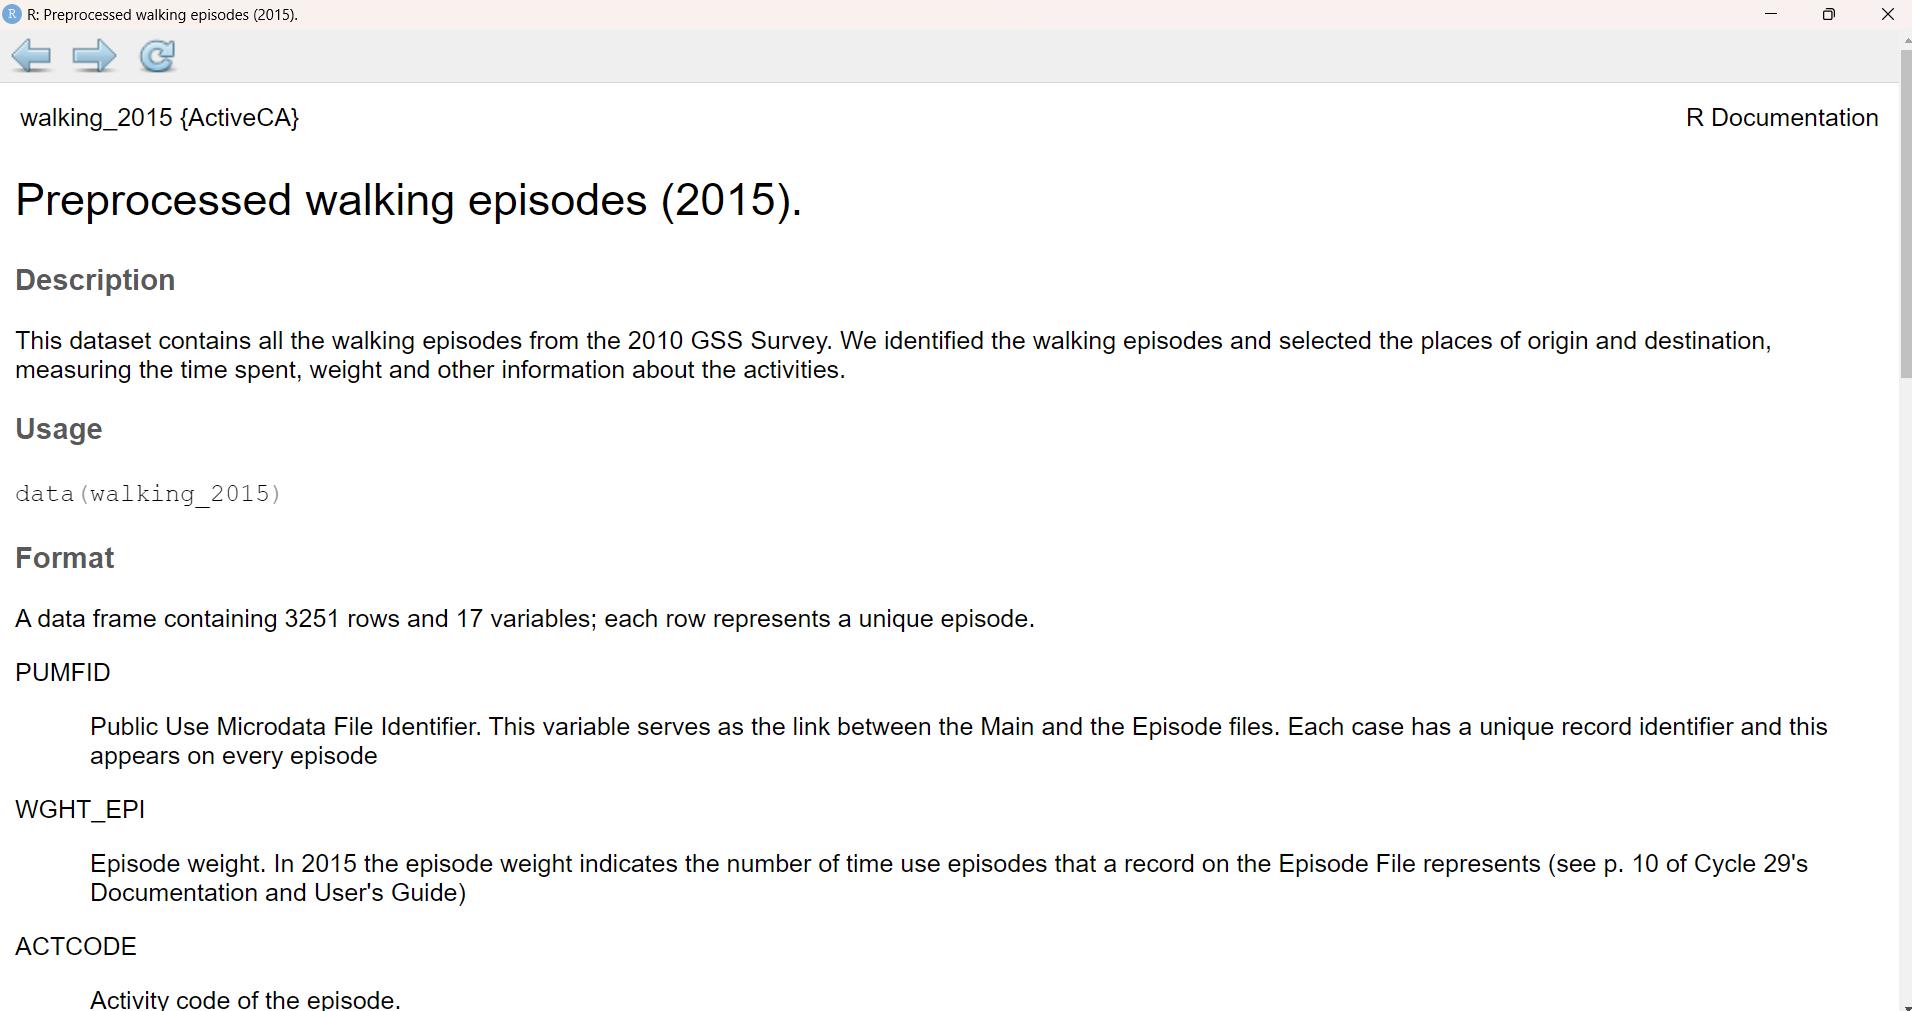
\includegraphics[width=1\linewidth]{Manuscript-figures/walking-2015-documentation} 
%DIFDELCMD < %%%
\DIFdelendFL \DIFaddbeginFL 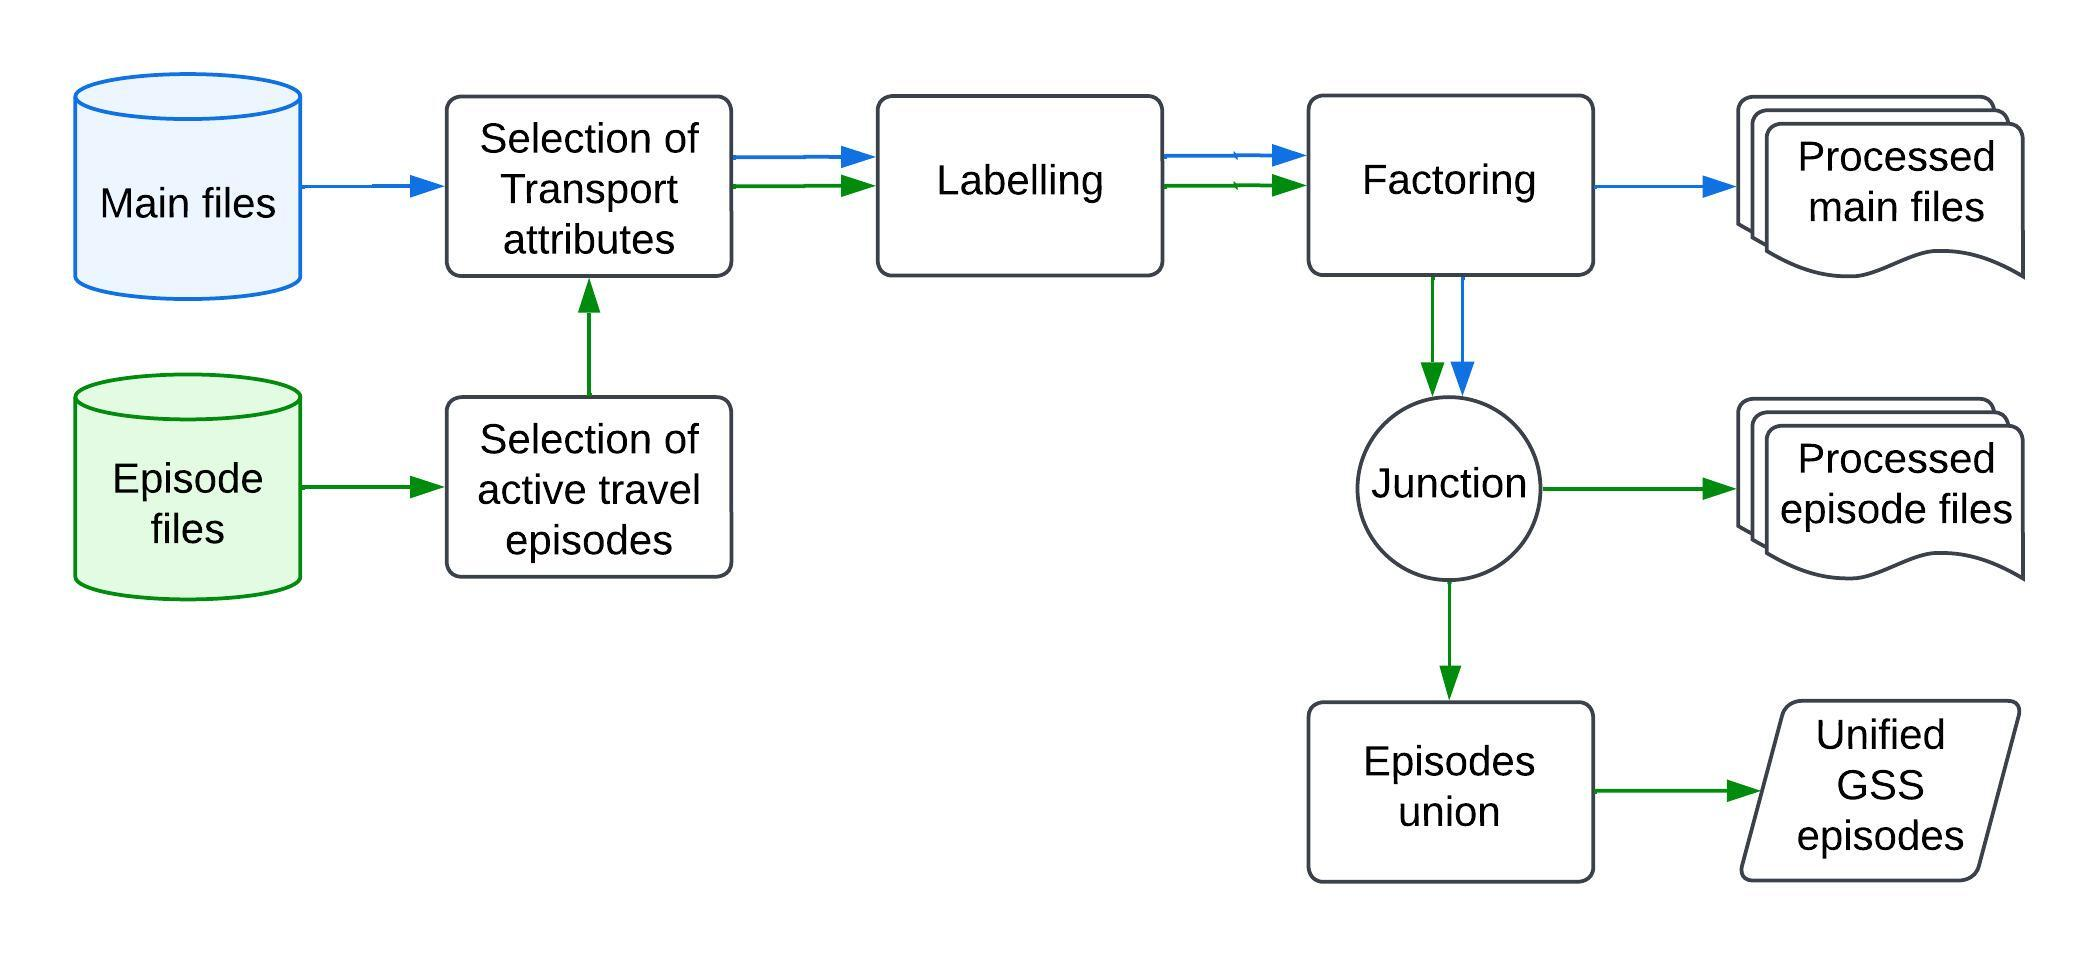
\includegraphics[width=1\linewidth]{Manuscript-figures/RPackages - ActiveCA} 
\DIFaddendFL 

}

\caption{\DIFdelbeginFL \DIFdelFL{Documentation for }\DIFdelendFL \DIFaddbeginFL \DIFaddFL{Diagram with }\DIFaddendFL the \DIFdelbeginFL \DIFdelFL{dataset of walking episodes from 2015.}\DIFdelendFL \DIFaddbeginFL \DIFaddFL{processes applied to the main (blue arrows) and episode files (green arrows) to obtain the ActiveCA datasets.}\DIFaddendFL }\DIFdelbeginFL %DIFDELCMD < \label{fig:walking_documentation}
%DIFDELCMD < %%%
\DIFdelendFL \DIFaddbeginFL \label{fig:process-figure}
\DIFaddendFL \end{figure}

\DIFdelbegin \DIFdel{The code below shows how to load the walking episodes from the 2015 GSS
(Cycle 29):
}\DIFdelend \DIFaddbegin \section{\DIFadd{\{ActiveCA\} data sets}}\label{activeca-data-sets}
\DIFaddend 

\DIFdelbegin %DIFDELCMD < \begin{verbatim}
%DIFDELCMD < %%%
%DIFAUXCMD NEXT
\DIFmodbegin
\begin{DIFverbatim}[alsolanguage=DIFcode]
%DIF < data(walking_2015)
\end{DIFverbatim}
\DIFmodend %DIFAUXCMD
%DIFDELCMD < \end{verbatim}
%DIFDELCMD < 

%DIFDELCMD < %%%
\DIFdel{The GSS surveys apply a probability sampling methodology, in which each
episode or person selected in the sample represents several other
episodes or persons not in the sample. The number of episodes and
persons represented by a episode or person is determined by the weight
or weighting factor. Because of this, estimates of the number of episodes or persons need to be calculated applying the corresponding
weighting factors.
}%DIFDELCMD < 

%DIFDELCMD < %%%
\DIFdel{For instance, to calculate the percentage of respondents from the 2015
GSS survey with active travel episodes, it is necessary to account for
the person's weight. In 2015, the weight variable is represented by
WGHT\_PER. The
code below demonstrates how to obtain the percentage of people with active travel episodes by age group. It uses the
dplyr
package \mbox{%DIFAUXCMD
\citep{dplyr2023} }\hskip0pt%DIFAUXCMD
to manipulate the data.
}%DIFDELCMD < 

%DIFDELCMD < %%%
\DIFdel{The process begins by creating a dataset that sums the population by age
group. Then, it joins the 2015 episodes with the 2015 Main File. Note
that in both operations, the code sums the person weight variable
(WGHT\_PER) to obtain the correct population values. After this,
a new
dataset, Active\_percentage, is created by merging both previous
datasets. The percentage of active travel episodes by age group is
calculated by dividing the total population by the population with
active trip episodes, then multiplying by 100 and rounding with 2
decimal places.
}%DIFDELCMD < 

%DIFDELCMD < \begin{verbatim}
%DIFDELCMD < %%%
%DIFAUXCMD NEXT
\DIFmodbegin
\begin{DIFverbatim}[alsolanguage=DIFcode]
%DIF < # Load the dplyr library for data manipulation
%DIF < library('dplyr')
%DIF < -
%DIF < # Load the episodes dataset
%DIF < data(gss_episodes) 
%DIF < -
%DIF < # Calculate the total population for each age group
%DIF < Total_population <- gss_main_2015 |> 
%DIF <   group_by(AGEGR10) |> 
%DIF <   summarise(Total_population  = sum(WGHT_PER))
%DIF < -
%DIF < # Calculate the active population for each age group
%DIF < Active_population <- gss_episodes |> 
%DIF <       filter(YEAR == 2015) |> 
%DIF <   left_join(gss_main_2015, by = c("PUMFID"="PUMFID")) |> 
%DIF <   group_by(AGEGR10) |> 
%DIF <   summarise(Active_population  = sum(WGHT_PER))
%DIF < -
%DIF < # Combine total and active population 
%DIF < #and calculate the percentage
%DIF < Active_percentage <- Total_population |> 
%DIF <   left_join(Active_population, by = c("AGEGR10" = "AGEGR10")) |>
%DIF <   mutate(
%DIF <     Percentage = round(Active_population/Total_population*100,2))
\end{DIFverbatim}
\DIFmodend %DIFAUXCMD
%DIFDELCMD < \end{verbatim}
%DIFDELCMD < 

%DIFDELCMD < %%%
\DIFdel{The result shows that the age group with the highest share of active
trips is those between 15 and 20 years old, with almost 37\%, followed
by those between 25 and 34 years old with around 33\%. There is a
significant drop in percentage for the following groups, with the
percentage falling to between 15\% and 18\% for the remaining age
groups}\DIFdelend \DIFaddbegin \DIFadd{This section presents some potential applications of the \{ActiveCA\}
}\texttt{\DIFadd{R}} \DIFadd{package. In fact, we expect that the application of this
package to extend beyond our pre-imagined range of uses. The
installation instruction and also some examples of application of the
\{ActiveCA\} }\texttt{\DIFadd{R}} \DIFadd{package are available in the }\texttt{\DIFadd{vignettes}}\DIFadd{,
available in the Github repository}\DIFaddend .

\DIFdelbegin %DIFDELCMD < \begin{longtable}[]{@{}lrrr@{}}
%DIFDELCMD < \toprule\noalign{}
%DIFDELCMD < AGEGR10 & Total\_population & Active\_population & Percentage \\
%DIFDELCMD < \midrule\noalign{}
%DIFDELCMD < \endhead
%DIFDELCMD < \bottomrule\noalign{}
%DIFDELCMD < \endlastfoot
%DIFDELCMD < 15 to 24 years & 4511131 & 1641468.3 & 36.39 \\
%DIFDELCMD < 25 to 34 years & 4956386 & 1644032.8 & 33.17 \\
%DIFDELCMD < 35 to 44 years & 4734506 & 847769.9 & 17.91 \\
%DIFDELCMD < 45 to 54 years & 5136125 & 790667.3 & 15.39 \\
%DIFDELCMD < 55 to 64 years & 4831306 & 767064.0 & 15.88 \\
%DIFDELCMD < 65 to 74 years & 3283969 & 559024.6 & 17.02 \\
%DIFDELCMD < 75 years and over & 2312976 & 384358.6 & 16.62 \\
%DIFDELCMD < \end{longtable}
%DIFDELCMD < %%%
\DIFdelend \DIFaddbegin \subsection{\DIFadd{Active episodes}}\label{active-episodes}
\DIFaddend 

\DIFdelbegin \subsection{\DIFdel{Processed data set}}%DIFAUXCMD
\addtocounter{subsection}{-1}%DIFAUXCMD
%DIFDELCMD < \label{processed-data-set}
%DIFDELCMD < 

%DIFDELCMD < %%%
\DIFdelend Table \ref{tab:processed-obs} displays the total number of records
processed for Main and \DIFdelbegin \DIFdel{Episode Files}\DIFdelend \DIFaddbegin \emph{\DIFadd{Episode files}}\DIFaddend . For the \DIFdelbegin \DIFdel{Main Files}\DIFdelend \DIFaddbegin \emph{\DIFadd{Main files}}\DIFaddend ,
a total of \DIFdelbegin \DIFdel{89,331 }\DIFdelend \DIFaddbegin \DIFadd{101,667 }\DIFaddend records were processed, referring to all records from
the Time Use Surveys from 1986 to \DIFdelbegin \DIFdel{2015}\DIFdelend \DIFaddbegin \DIFadd{2022}\DIFaddend , that together represents more of
\DIFdelbegin \DIFdel{149,389,839 respondents(29,766,399 for 2015, 28,075,610 for 2010,
26,095,819 for 2005, 24,260,137 for 1998, 21,294,313 for 1992, and for
2005, 24,260,137 for 1998, and 21,294,313 for 1986)}\DIFdelend \DIFaddbegin \DIFadd{181,526,641 respondents}\DIFaddend . It also presents the total cases of active
trips episodes identified. In total 23,513 records with register of
active travel activity. Together, these records account for 44,316,110
episodes.

\begingroup\DIFdelbegin %DIFDELCMD < \fontsize{10}{12}%%%
\DIFdelend \DIFaddbegin \fontsize{8}{10}\DIFaddend \selectfont

\DIFdelbegin %DIFDELCMD < \begin{longtable}[t]{lrrr}
%DIFDELCMD < \caption{\label{tab:table_df_processed}\label{tab:processed-obs}Total number and weighted sum of records processed.}\\
%DIFDELCMD < \toprule
%DIFDELCMD < \multicolumn{2}{c}{ } & \multicolumn{2}{c}{Observations} \\
%DIFDELCMD < \cmidrule(l{3pt}r{3pt}){3-4}
%DIFDELCMD < Survey & Year & Count & Weighted\\
%DIFDELCMD < \midrule
%DIFDELCMD <  & 2015 & 17390 & 29766399\\
%DIFDELCMD < \nopagebreak
%DIFDELCMD <  & 2010 & 15390 & 28075610\\
%DIFDELCMD < \nopagebreak
%DIFDELCMD <  & 2005 & 19597 & 26095819\\
%DIFDELCMD < \nopagebreak
%DIFDELCMD <  & 1998 & 10749 & 24260137\\
%DIFDELCMD < \nopagebreak
%DIFDELCMD <  & 1992 & 9815 & 21294313\\
%DIFDELCMD < \nopagebreak
%DIFDELCMD < \multirow[t]{-6}{*}{\raggedright\arraybackslash Main} & 1986 & 16390 & 19897562\\
%DIFDELCMD < \cmidrule{1-4}\pagebreak[0]
%DIFDELCMD <  & 2022 & 1765 & 6041032\\
%DIFDELCMD < \nopagebreak
%DIFDELCMD <  & 2015 & 3496 & 6634387\\
%DIFDELCMD < \nopagebreak
%DIFDELCMD <  & 2010 & 4615 & 8516753\\
%DIFDELCMD < \nopagebreak
%DIFDELCMD <  & 2005 & 5866 & 7583838\\
%DIFDELCMD < \nopagebreak
%DIFDELCMD <  & 1998 & 1789 & 3606987\\
%DIFDELCMD < \nopagebreak
%DIFDELCMD <  & 1992 & 1635 & 3691918\\
%DIFDELCMD < \nopagebreak
%DIFDELCMD < \multirow[t]{-7}{*}{\raggedright\arraybackslash Episode} & 1986 & 4347 & 8241196\\
%DIFDELCMD < \bottomrule
%DIFDELCMD < \end{longtable}
%DIFDELCMD < %%%
\DIFdelend \DIFaddbegin \begin{longtable}[t]{rr>{}r|rr}
\caption{\label{tab:table_df_processed}\label{tab:processed-obs}Total number and weighted sum of records processed.}\\
\toprule
\multicolumn{1}{c}{ } & \multicolumn{2}{c}{Main} & \multicolumn{2}{c}{Episode} \\
\cmidrule(l{3pt}r{3pt}){2-3} \cmidrule(l{3pt}r{3pt}){4-5}
Year & Count & Weighted & Count\_ep & Weighted\_ep\\
\midrule
2022 & 12336 & 32136802 & 1765 & 6041032\\
2015 & 17390 & 29766399 & 3496 & 6634387\\
2010 & 15390 & 28075610 & 4615 & 8516753\\
2005 & 19597 & 26095819 & 5866 & 7583838\\
1998 & 10749 & 24260137 & 1789 & 3606987\\
\addlinespace
1992 & 9815 & 21294313 & 1635 & 3691918\\
1986 & 16390 & 19897562 & 4347 & 8241196\\
\bottomrule
\end{longtable}
\DIFaddend \endgroup{}

Table \ref{tab:main-2015-processed} shows the first ten rows and first
six variables of the \DIFdelbegin \DIFdel{GSS }\DIFdelend \DIFaddbegin \DIFadd{TUS }\DIFaddend PUMF 2015 Main File (Cycle 29), displayed in
\ref{tab:main-2015-unprocessed} before our processing. Table
\ref{tab:ep-2015-processed} presents the walking episodes for the record
identification number \DIFdelbegin \DIFdel{10041 from the GSS }\DIFdelend \DIFaddbegin \texttt{\DIFadd{10041}} \DIFadd{from the TUS }\DIFaddend PUMF 2015
\DIFdelbegin \DIFdel{Episode File }\DIFdelend \DIFaddbegin \emph{\DIFadd{Episode file}} \DIFaddend (Cycle 29), previously displayed in Table
\ref{tab:ep-2015-unprocessed}. Only the unique active travel episode
appear in Table \ref{tab:ep-2015-processed} since the records were
filtered to select cases with walking or cycling episodes. For both
cases, Tables \ref{tab:main-2015-processed} and
\ref{tab:ep-2015-processed} contain labeled variables, facilitating the
interpretation of the data.

\begingroup\fontsize{8}{10}\selectfont

\begin{ThreePartTable}
\begin{TableNotes}
\item \textit{Note: } 
\item Legend: \DIFdelbegin \DIFdel{`PUMFID`}\DIFdelend \DIFaddbegin \DIFadd{PUMFID}\DIFaddend : record identification. \DIFdelbegin \DIFdel{`}\DIFdelend WGHT\_PER\DIFdelbegin \DIFdel{`}\DIFdelend :  person weight. \DIFdelbegin \DIFdel{`SURVMNTH`}\DIFdelend \DIFaddbegin \DIFadd{SURVMNTH}\DIFaddend : survey month of data collection. \DIFdelbegin \DIFdel{`}\DIFdelend AGEGR10\DIFdelbegin \DIFdel{`}\DIFdelend : age group of the respondent. \DIFdelbegin \DIFdel{`SEX`}\DIFdelend \DIFaddbegin \DIFadd{SEX}\DIFaddend : sex of the respondent. \DIFdelbegin \DIFdel{`MARSTAT`}\DIFdelend \DIFaddbegin \DIFadd{MARSTAT}\DIFaddend : marital status of the respondent.
\end{TableNotes}
\DIFdelbegin %DIFDELCMD < \begin{longtable}[t]{cccccc}
%DIFDELCMD < \caption{\label{tab:gss-processed-file-2015}\label{tab:main-2015-processed}Visualization of the first ten lines and first six columns of the Main File of the 2015 GSS.}\\
%DIFDELCMD < \toprule
%DIFDELCMD < PUMFID & WGHT\_PER & SURVMNTH & AGEGR10 & SEX & MARSTAT\\
%DIFDELCMD < \midrule
%DIFDELCMD < 10000 & 616.6740 & July & 55 to 64 years & Male & Divorced\\
%DIFDELCMD < 10001 & 8516.6140 & July & 55 to 64 years & Male & Married\\
%DIFDELCMD < 10002 & 371.7520 & January & 45 to 54 years & Female & Married\\
%DIFDELCMD < 10003 & 1019.3135 & March & 65 to 74 years & Female & Divorced\\
%DIFDELCMD < 10004 & 1916.0708 & September & 25 to 34 years & Male & Single, never married\\
%DIFDELCMD < \addlinespace
%DIFDELCMD < 10005 & 1952.2015 & April & 15 to 24 years & Male & Single, never married\\
%DIFDELCMD < 10006 & 5761.5528 & August & 15 to 24 years & Male & Single, never married\\
%DIFDELCMD < 10007 & 466.0426 & June & 55 to 64 years & Female & Widowed\\
%DIFDELCMD < 10008 & 2479.2991 & February & 25 to 34 years & Female & Married\\
%DIFDELCMD < 10009 & 1436.1641 & August & 65 to 74 years & Male & Widowed\\
%DIFDELCMD < \bottomrule
%DIFDELCMD < \insertTableNotes
%DIFDELCMD < \end{longtable}
%DIFDELCMD < %%%
\DIFdelend \DIFaddbegin \begin{longtable}[t]{cccccc}
\caption{\label{tab:gss-processed-file-2015}\label{tab:main-2015-processed}Visualization of the first ten lines and first six columns of the 2015 TUS Main File.}\\
\toprule
PUMFID & WGHT\_PER & SURVMNTH & AGEGR10 & SEX & MARSTAT\\
\midrule
10000 & 616.6740 & July & 55 to 64 years & Male & Divorced\\
10001 & 8516.6140 & July & 55 to 64 years & Male & Married\\
10002 & 371.7520 & January & 45 to 54 years & Female & Married\\
10003 & 1019.3135 & March & 65 to 74 years & Female & Divorced\\
10004 & 1916.0708 & September & 25 to 34 years & Male & Single, never married\\
\addlinespace
10005 & 1952.2015 & April & 15 to 24 years & Male & Single, never married\\
10006 & 5761.5528 & August & 15 to 24 years & Male & Single, never married\\
10007 & 466.0426 & June & 55 to 64 years & Female & Widowed\\
10008 & 2479.2991 & February & 25 to 34 years & Female & Married\\
10009 & 1436.1641 & August & 65 to 74 years & Male & Widowed\\
\bottomrule
\insertTableNotes
\end{longtable}
\DIFaddend \end{ThreePartTable}
\endgroup{}

\begingroup\fontsize{8}{10}\selectfont

\begin{ThreePartTable}
\begin{TableNotes}
\item \textit{Note: } 
\item Legend: \DIFdelbegin \DIFdel{`PUMFID`}\DIFdelend \DIFaddbegin \DIFadd{PUMFID}\DIFaddend : record identification. \DIFdelbegin \DIFdel{`EPINO`}\DIFdelend \DIFaddbegin \DIFadd{EPINO}\DIFaddend : episode number. WGHT\_EPI: episode's weight. TUI\_01: activity code. DURATION: episode's duration. LOCATION: episode's location.
\end{TableNotes}
\DIFdelbegin %DIFDELCMD < \begin{longtable}[t]{rrlrlll}
%DIFDELCMD < \caption{\label{tab:gss-processed-file-2015}\label{tab:ep-2015-processed}Visualization of the active travel episode for the record number `10041` of the 2015 GSS survey.}\\
%DIFDELCMD < \toprule
%DIFDELCMD < PUMFID & WGHT\_EPI & Activity & Duration & Origin & Destination & Mode\\
%DIFDELCMD < \midrule
%DIFDELCMD < 10041 & 1353.818 & Transport to or from activity & 15 & Home & Home & Walking\\
%DIFDELCMD < \bottomrule
%DIFDELCMD < \insertTableNotes
%DIFDELCMD < \end{longtable}
%DIFDELCMD < %%%
\DIFdelend \DIFaddbegin \begin{longtable}[t]{rrlrlll}
\caption{\label{tab:gss-processed-file-2015}\label{tab:ep-2015-processed}Visualization of the active travel episode for the record number 10041 of the 2015 GSS survey.}\\
\toprule
PUMFID & WGHT\_EPI & Activity & Duration & Origin & Destination & Mode\\
\midrule
10041 & 1353.818 & Transport to or from activity & 15 & Home & Home & Walking\\
\bottomrule
\insertTableNotes
\end{longtable}
\DIFaddend \end{ThreePartTable}
\endgroup{}

\subsection{Descriptive statistics}\label{descriptive-statistics}

Considering \DIFdelbegin \DIFdel{GSS Cycles }\DIFdelend \DIFaddbegin \DIFadd{all TUS }\DIFaddend analyzed, we identified 23,513 episodes that
recorded active travel episodes, with trip duration ranging from 0 to
900 minutes, to twelve different destinations. \{ActiveCA\} includes all
these episodes ready for analysis. Table \ref{tab:table-01} presents
descriptive statistics on walking and cycling trips between 1986 and
\DIFdelbegin \DIFdel{2015}\DIFdelend \DIFaddbegin \DIFadd{2022}\DIFaddend , with measures of trip duration in minutes. The 1986 survey did not
include bicycle trips.

\begingroup\DIFdelbegin %DIFDELCMD < \fontsize{10}{12}%%%
\DIFdelend \DIFaddbegin \fontsize{8}{10}\DIFaddend \selectfont

\begin{longtable}[t]{>{}llccccccc}
\caption{\label{tab:table-01}\label{tab:table-01}Descriptive statistics for episodes with active transport records}\\
\toprule
\multicolumn{2}{c}{ } & \multicolumn{7}{c}{Year} \\
\cmidrule(l{3pt}r{3pt}){3-9}
Mode & Statistic & 1986 & 1992 & 1998 & 2005 & 2010 & 2015 & 2022\\
\midrule
 & Maximum & 660 & 300 & 255 & 515 & 480 & 900 & 480\\
\nopagebreak
 & Mean & 21 & 21 & 12 & 12 & 13 & 18 & 19\\
\nopagebreak
 & Median & 15 & 10 & 5 & 10 & 10 & 10 & 15\\
\nopagebreak
 & Minimum & 1 & 1 & 1 & 0 & 0 & 5 & 5\\
\nopagebreak
\multirow[t]{-5}{*}{\raggedright\arraybackslash \textbf{Walking}} & Standard deviation & 31 & 25 & 17 & 16 & 17 & 27 & 24\\
\cmidrule{1-9}\pagebreak[0]
 & Maximum &  & 240 & 90 & 180 & 153 & 120 & 150\\
\nopagebreak
 & Mean &  & 28 & 24 & 20 & 19 & 25 & 40\\
\nopagebreak
 & Median &  & 15 & 15 & 15 & 10 & 20 & 30\\
\nopagebreak
 & Minimum &  & 5 & 2 & 1 & 1 & 5 & 5\\
\nopagebreak
\multirow[t]{-5}{*}{\raggedright\arraybackslash \textbf{Cycling}} & Standard deviation &  & 36 & 18 & 18 & 23 & 20 & 20\\
\bottomrule
\end{longtable}
\endgroup{}

Table \ref{tab:table-01} shows that, \DIFdelbegin \DIFdel{in general, }\DIFdelend \DIFaddbegin \DIFadd{until 2022 }\DIFaddend the median values for
walking trips \DIFdelbegin \DIFdel{is }\DIFdelend \DIFaddbegin \DIFadd{were }\DIFaddend 10 minutes, \DIFdelbegin \DIFdel{except for 1998 when the median was 5
minutes }\DIFdelend \DIFaddbegin \DIFadd{increasing to 15 minutes in the last
survey}\DIFaddend . In the case of cycling trips, the duration fluctuated over the
years, ranging from 10 to \DIFdelbegin \DIFdel{20 }\DIFdelend \DIFaddbegin \DIFadd{30 }\DIFaddend minutes. The table also highlights very
high maximum values, particularly for walking trips, with recorded
episodes exceeding 4 hours in all cases.

\DIFdelbegin \DIFdel{Table \ref{tab:table-02} and \ref{tab:table-03} provide descriptive
statistics for the two modes of transportation, split by destination
categories, from 1986 to 1998 and from 2005 to 2015, respectively. In
Table \ref{tab:table-02}, one can observed that in 1986 and 1992,
walking trips destined for home had the highest medians. However, by
1998, the highest medians shifted to trips to work or school, a
transition that also occurred for cycling trips between 1992 and 1998.
Table \ref{tab:table-03} indicates that the median duration for walking
trips to home and work or school remained at 10 minutes.
}%DIFDELCMD < 

%DIFDELCMD < \begingroup\fontsize{6}{8}\selectfont
%DIFDELCMD < 

%DIFDELCMD < \begin{ThreePartTable}
%DIFDELCMD < \begin{TableNotes}
%DIFDELCMD < \item %%%
\textit{\DIFdel{Note: }} 
%DIFAUXCMD
%DIFDELCMD < \item %%%
\DIFdel{'Min' denotes the minimum time to reach the destination; 'Max' denotes the maximum time to reach the destination; '(\%)' indicates a percentage of the total time to reach the destination; 'Med' refers to the median time to reach the destination
}%DIFDELCMD < \end{TableNotes}
%DIFDELCMD < \begin{longtable}[t]{ccccc>{}c|ccc>{}c|cccc}
%DIFDELCMD < \caption{\label{tab:table-02}\label{tab:table-02}Comparison of travel statistics by mode and destination: 1986, 1992, 1998}\\
%DIFDELCMD < \toprule
%DIFDELCMD < \multicolumn{2}{c}{ } & \multicolumn{4}{c}{1986} & \multicolumn{4}{c}{1992} & \multicolumn{4}{c}{1998} \\
%DIFDELCMD < \cmidrule(l{3pt}r{3pt}){3-6} \cmidrule(l{3pt}r{3pt}){7-10} \cmidrule(l{3pt}r{3pt}){11-14}
%DIFDELCMD < \multicolumn{1}{c}{\textbf{Destination}} & \multicolumn{1}{c}{\textbf{Mode}} & \multicolumn{1}{c}{\textbf{Min}} & \multicolumn{1}{c}{\textbf{Med}} & \multicolumn{1}{c}{\textbf{Max}} & \multicolumn{1}{c}{\textbf{(\%)}} & \multicolumn{1}{c}{\textbf{Min}} & \multicolumn{1}{c}{\textbf{Med}} & \multicolumn{1}{c}{\textbf{Max}} & \multicolumn{1}{c}{\textbf{(\%)}} & \multicolumn{1}{c}{\textbf{Min}} & \multicolumn{1}{c}{\textbf{Med}} & \multicolumn{1}{c}{\textbf{Max}} & \multicolumn{1}{c}{\textbf{(\%)}}\\
%DIFDELCMD < \midrule
%DIFDELCMD <  & Home &  &  &  &  & 5 & 20 & 240 & 55.7 & 2 & 15 & 90 & 51.6\\
%DIFDELCMD < \nopagebreak
%DIFDELCMD <  & Other's home &  &  &  &  & 5 & 10 & 145 & 19.7 & 2 & 10 & 80 & 15.7\\
%DIFDELCMD < \nopagebreak
%DIFDELCMD < \multirow[t]{-3}{*}{\centering\arraybackslash Cycling} & Work or school &  &  &  &  & 5 & 15 & 45 & 24.7 & 5 & 25 & 75 & 32.8\\
%DIFDELCMD < \cmidrule{1-14}\pagebreak[0]
%DIFDELCMD <  & Home & 1 & 15 & 330 & 46.3 & 1 & 15 & 300 & 60.5 & 1 & 5 & 255 & 51.9\\
%DIFDELCMD < \nopagebreak
%DIFDELCMD <  & Other's home & 1 & 10 & 660 & 42.6 & 1 & 5 & 135 & 18.7 & 1 & 5 & 120 & 27.8\\
%DIFDELCMD < \nopagebreak
%DIFDELCMD < \multirow[t]{-3}{*}{\centering\arraybackslash Walking} & Work or school & 1 & 10 & 450 & 11.1 & 2 & 10 & 60 & 20.9 & 1 & 10 & 75 & 20.3\\
%DIFDELCMD < \bottomrule
%DIFDELCMD < \insertTableNotes
%DIFDELCMD < \end{longtable}
%DIFDELCMD < \end{ThreePartTable}
%DIFDELCMD < \endgroup{}
%DIFDELCMD < 

%DIFDELCMD < \begingroup\fontsize{6}{8}\selectfont
%DIFDELCMD < 

%DIFDELCMD < \begin{ThreePartTable}
%DIFDELCMD < \begin{TableNotes}
%DIFDELCMD < \item %%%
\textit{\DIFdel{Note: }} 
%DIFAUXCMD
%DIFDELCMD < \item %%%
\DIFdel{'Min' denotes the minimum time to reach the destination; 'Max' denotes the maximum time to reach the destination; '(\%)' indicates a percentage of the total time to reach the destination; 'Med' refers to the median time to reach the destination
}%DIFDELCMD < \end{TableNotes}
%DIFDELCMD < \begin{longtable}[t]{ccccc>{}c|ccc>{}c|cccc}
%DIFDELCMD < \caption{\label{tab:table-03}\label{tab:table-03}Comparison of travel statistics by mode and destination: 2005, 2010, 2015}\\
%DIFDELCMD < \toprule
%DIFDELCMD < \multicolumn{2}{c}{ } & \multicolumn{4}{c}{2005} & \multicolumn{4}{c}{2010} & \multicolumn{4}{c}{2015} \\
%DIFDELCMD < \cmidrule(l{3pt}r{3pt}){3-6} \cmidrule(l{3pt}r{3pt}){7-10} \cmidrule(l{3pt}r{3pt}){11-14}
%DIFDELCMD < \multicolumn{1}{c}{\textbf{Destination}} & \multicolumn{1}{c}{\textbf{Mode}} & \multicolumn{1}{c}{\textbf{Min}} & \multicolumn{1}{c}{\textbf{Med}} & \multicolumn{1}{c}{\textbf{Max}} & \multicolumn{1}{c}{\textbf{(\%)}} & \multicolumn{1}{c}{\textbf{Min}} & \multicolumn{1}{c}{\textbf{Med}} & \multicolumn{1}{c}{\textbf{Max}} & \multicolumn{1}{c}{\textbf{(\%)}} & \multicolumn{1}{c}{\textbf{Min}} & \multicolumn{1}{c}{\textbf{Med}} & \multicolumn{1}{c}{\textbf{Max}} & \multicolumn{1}{c}{\textbf{(\%)}}\\
%DIFDELCMD < \midrule
%DIFDELCMD <  & Cultural venues & 10 & 10 & 15 & 0.3 & 10 & 25 & 30 & 1.0 & 15 & 15 & 15 & 0.5\\
%DIFDELCMD < \nopagebreak
%DIFDELCMD <  & Grocery store & 2 & 10 & 30 & 10.4 & 5 & 10 & 75 & 7.2 & 5 & 15 & 80 & 5.5\\
%DIFDELCMD < \nopagebreak
%DIFDELCMD <  & Health clinic &  &  &  &  &  &  &  &  & 10 & 15 & 90 & 1.9\\
%DIFDELCMD < \nopagebreak
%DIFDELCMD <  & Home & 1 & 15 & 180 & 48.4 & 1 & 10 & 135 & 48.8 & 5 & 20 & 120 & 46.4\\
%DIFDELCMD < \nopagebreak
%DIFDELCMD <  & Neighbourhood &  &  &  &  &  &  &  &  & 10 & 30 & 45 & 1.3\\
%DIFDELCMD < \nopagebreak
%DIFDELCMD <  & Other's home & 1 & 10 & 35 & 9.4 & 5 & 10 & 45 & 9.7 & 5 & 15 & 40 & 4.8\\
%DIFDELCMD < \nopagebreak
%DIFDELCMD <  & Outdoors & 5 & 15 & 45 & 6.0 & 3 & 10 & 115 & 2.6 & 15 & 30 & 30 & 1.0\\
%DIFDELCMD < \nopagebreak
%DIFDELCMD <  & Place of worship & 20 & 20 & 20 & 0.1 &  &  &  &  & 15 & 15 & 15 & 0.2\\
%DIFDELCMD < \nopagebreak
%DIFDELCMD <  & Restaurant & 5 & 15 & 35 & 2.8 & 10 & 15 & 153 & 1.7 & 10 & 20 & 60 & 3.0\\
%DIFDELCMD < \nopagebreak
%DIFDELCMD <  & Sport area &  &  &  &  &  &  &  &  & 10 & 15 & 15 & 2.0\\
%DIFDELCMD < \nopagebreak
%DIFDELCMD < \multirow[t]{-11}{*}{\centering\arraybackslash Cycling} & Work or school & 1 & 15 & 90 & 22.6 & 1 & 15 & 100 & 29.0 & 5 & 20 & 120 & 33.5\\
%DIFDELCMD < \cmidrule{1-14}\pagebreak[0]
%DIFDELCMD <  & Business &  &  &  &  &  &  &  &  & 5 & 10 & 30 & 0.2\\
%DIFDELCMD < \nopagebreak
%DIFDELCMD <  & Cultural venues & 5 & 10 & 40 & 0.6 & 2 & 10 & 40 & 0.7 & 5 & 15 & 40 & 1.5\\
%DIFDELCMD < \nopagebreak
%DIFDELCMD <  & Grocery store & 1 & 10 & 90 & 11.5 & 1 & 7 & 105 & 13.1 & 5 & 10 & 130 & 10.3\\
%DIFDELCMD < \nopagebreak
%DIFDELCMD <  & Health clinic &  &  &  &  &  &  &  &  & 5 & 10 & 130 & 0.9\\
%DIFDELCMD < \nopagebreak
%DIFDELCMD <  & Home & 0 & 10 & 515 & 43.0 & 0 & 10 & 270 & 41.4 & 5 & 10 & 900 & 44.0\\
%DIFDELCMD < \nopagebreak
%DIFDELCMD <  & Neighbourhood &  &  &  &  &  &  &  &  & 5 & 10 & 60 & 2.6\\
%DIFDELCMD < \nopagebreak
%DIFDELCMD <  & Other's home & 1 & 5 & 300 & 10.2 & 0 & 5 & 140 & 10.2 & 5 & 10 & 120 & 6.2\\
%DIFDELCMD < \nopagebreak
%DIFDELCMD <  & Outdoors & 1 & 5 & 295 & 3.4 & 0 & 10 & 480 & 5.0 & 5 & 10 & 135 & 3.1\\
%DIFDELCMD < \nopagebreak
%DIFDELCMD <  & Place of worship & 1 & 10 & 30 & 0.7 & 1 & 7 & 60 & 0.8 & 5 & 15 & 45 & 1.1\\
%DIFDELCMD < \nopagebreak
%DIFDELCMD <  & Restaurant & 0 & 5 & 85 & 9.9 & 1 & 7 & 153 & 11.0 & 5 & 10 & 120 & 9.0\\
%DIFDELCMD < \nopagebreak
%DIFDELCMD <  & Sport area &  &  &  &  &  &  &  &  & 5 & 10 & 45 & 3.3\\
%DIFDELCMD < \nopagebreak
%DIFDELCMD < \multirow[t]{-12}{*}{\centering\arraybackslash Walking} & Work or school & 0 & 10 & 175 & 20.7 & 0 & 10 & 150 & 17.9 & 5 & 10 & 190 & 17.8\\
%DIFDELCMD < \bottomrule
%DIFDELCMD < \insertTableNotes
%DIFDELCMD < \end{longtable}
%DIFDELCMD < \end{ThreePartTable}
%DIFDELCMD < \endgroup{}
%DIFDELCMD < 

%DIFDELCMD < %%%
\DIFdelend \{ActiveCA\} also enables visual analysis of active travel in Canada
using \DIFdelbegin \DIFdel{traditional }\DIFdelend exploratory data analysis techniques. \DIFdelbegin \DIFdel{Figures
\ref{fig:figure-01}
and \ref{fig:figure-02} show walking and cycling
trips from 1992 and 2015 }\DIFdelend \DIFaddbegin \DIFadd{Figure \ref{fig:figure-01}
shows walking trips from 2022 }\DIFaddend through heat maps. \DIFdelbegin \DIFdel{These maps use }\DIFdelend \DIFaddbegin \DIFadd{This graph uses }\DIFaddend color
gradients to represent the percentage of trips between various origins
and destinations, with darker colors indicating higher percentages and
lighter colors representing less frequent routes. For conciseness, we
omitted the heat maps for the other years analyzed.

In \DIFdelbegin \DIFdel{1992, walking trips with home as both the origin and destination made
up the majority, accounting for about 30\% of all walking trips. These
trips often involved leisure activities, like short walks or dog
walking. Following this, trips from home to work or school comprised
18\% of walking trips. Overall, home emerged as a crucial hub, either as
an origin or destination, with only 5\% of trips not involving home. By
2015, home remained a significant node, but new locations distributed
the proportion of trips to areas not considered in 1992. In 2015, the
highest proportion of trips were from home to
work or school (12}\DIFdelend \DIFaddbegin \DIFadd{2022, }\texttt{\DIFadd{home}} \DIFadd{served as a central hub for most trips, with
fewer than 10\% of journeys not involving it as either a starting point
or destination. The most common trip types were from }\texttt{\DIFadd{home}} \DIFadd{to
}\texttt{\DIFadd{work\ or\ school}} \DIFadd{(17}\DIFaddend \%) and \DIFdelbegin \DIFdel{vice versa (11}\DIFdelend \DIFaddbegin \DIFadd{the reverse, from
}\texttt{\DIFadd{work\ or\ school}} \DIFadd{to }\texttt{\DIFadd{home}} \DIFadd{(13}\DIFaddend \%). \DIFdelbegin \DIFdel{home to home accounted for 8}\DIFdelend \DIFaddbegin \DIFadd{Notably, 7}\DIFaddend \% of trips
\DIFdelbegin \DIFdel{, and grocery
stores became a
notable destinationfor those leaving home (6\%), surpassing trips to other's home (4\% ).
}\DIFdelend \DIFaddbegin \DIFadd{began and ended at }\texttt{\DIFadd{home}}\DIFadd{, often reflecting leisure activities
such as short walks or dog walking. }\texttt{\DIFadd{Grocery\ stores}} \DIFadd{were also a
key destination, comprising 10\% of trips departing from }\texttt{\DIFadd{home.}}
\DIFaddend 

\begin{figure}

{\centering \DIFdelbeginFL %DIFDELCMD < 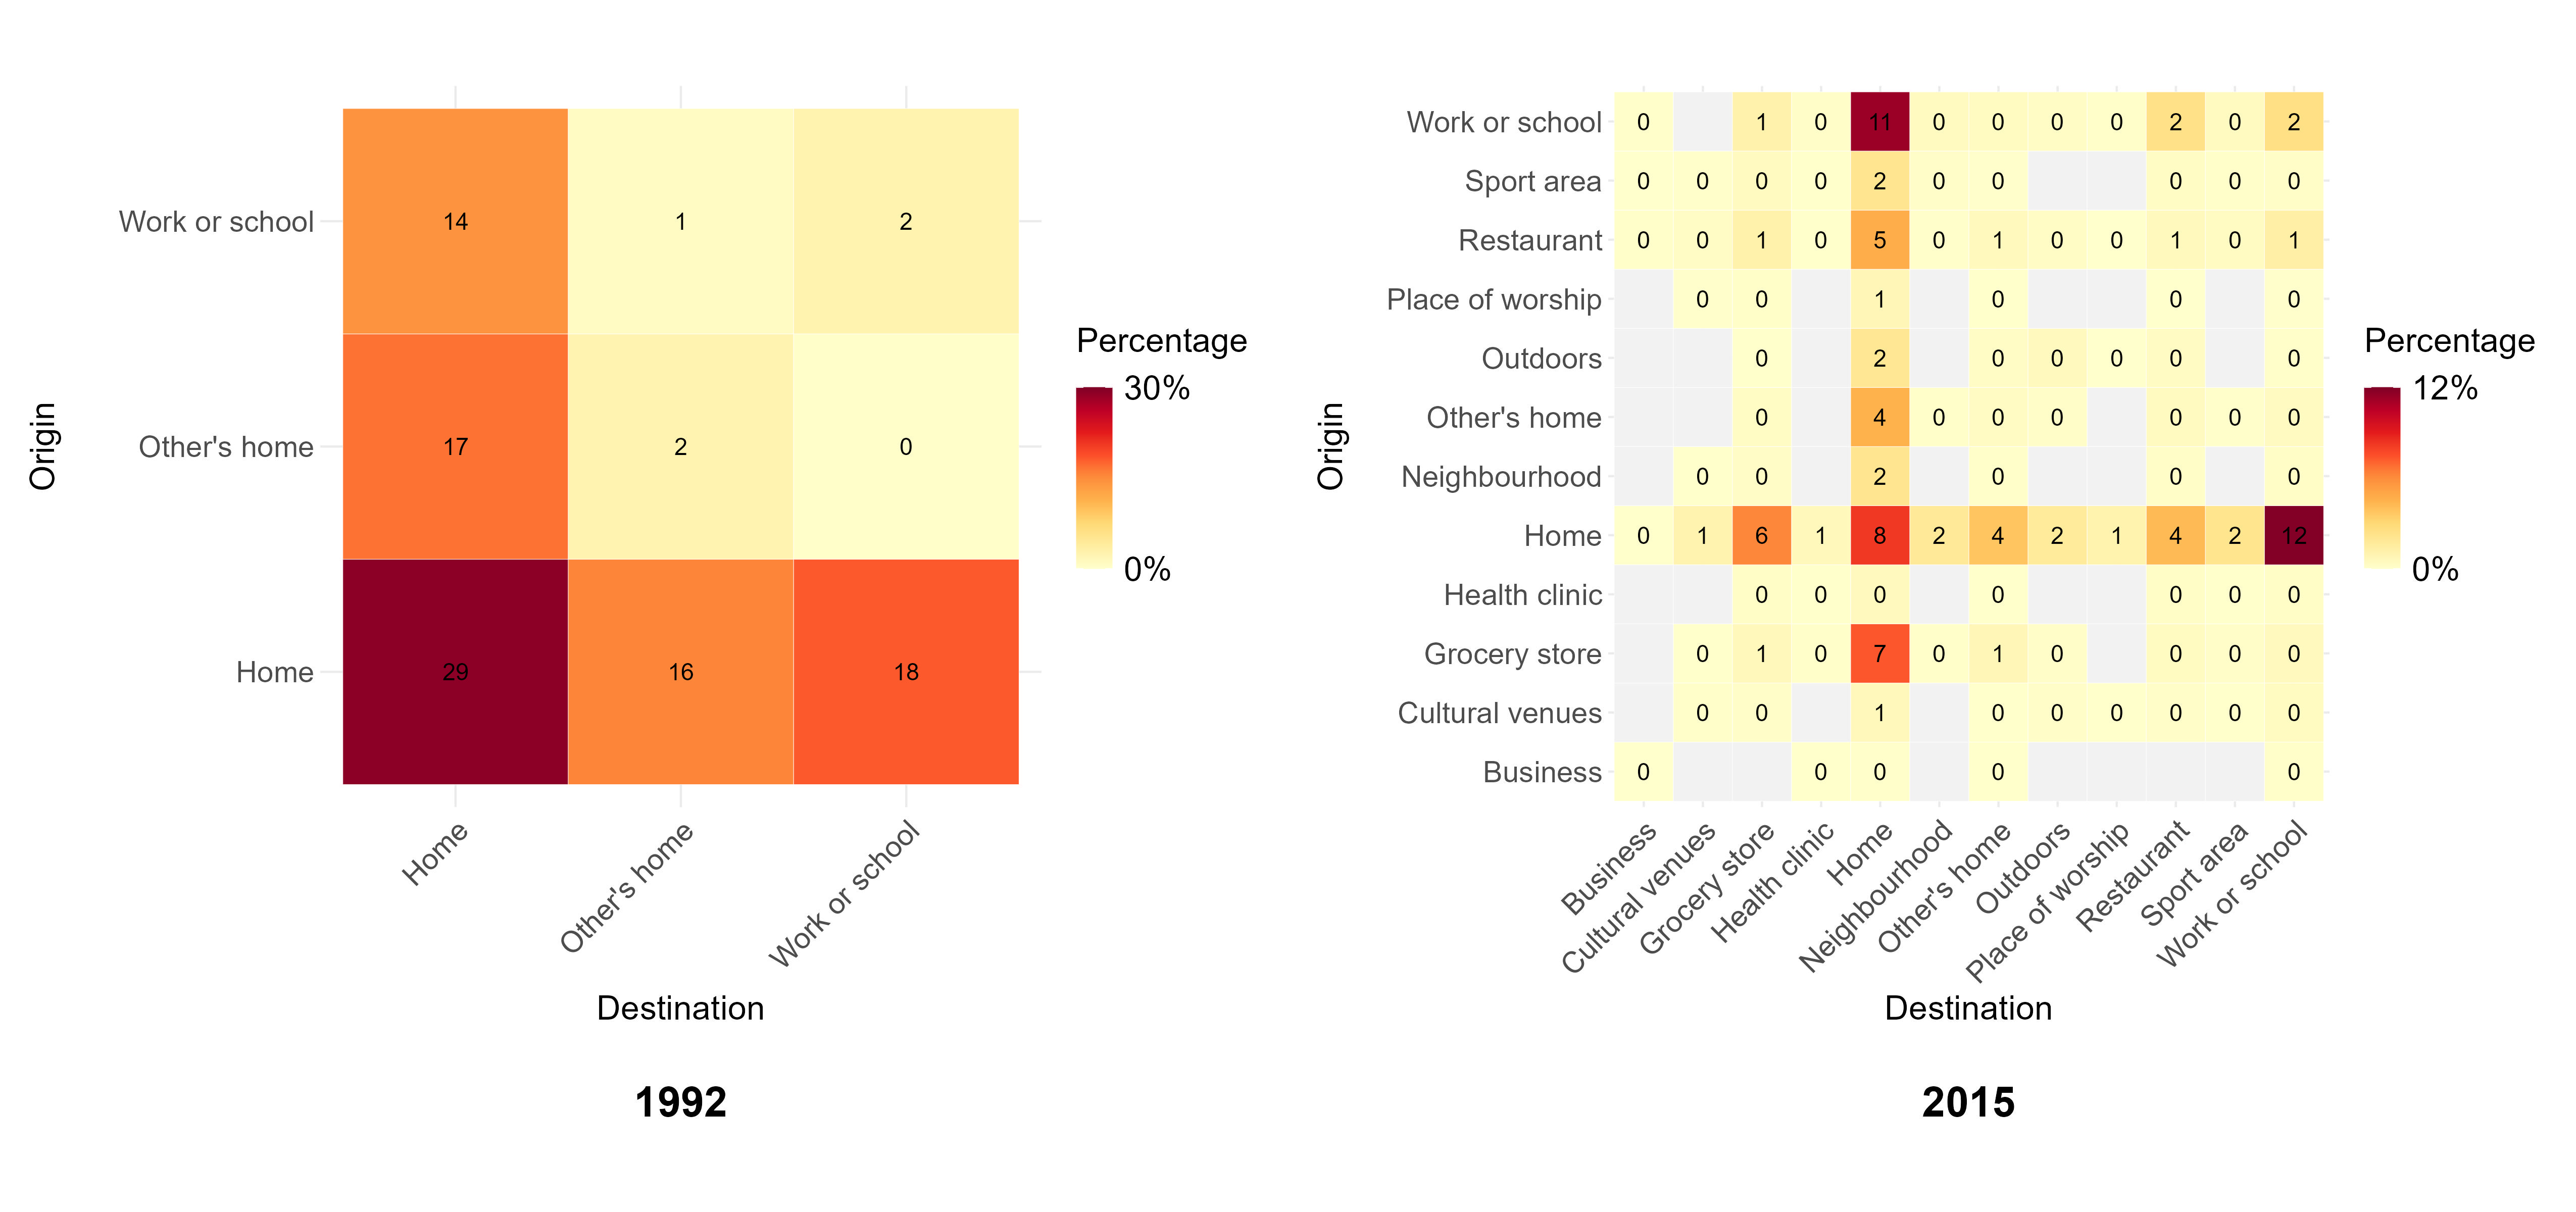
\includegraphics[width=1\linewidth]{Manuscript-figures/walking_hm_fig} 
%DIFDELCMD < %%%
\DIFdelendFL \DIFaddbeginFL 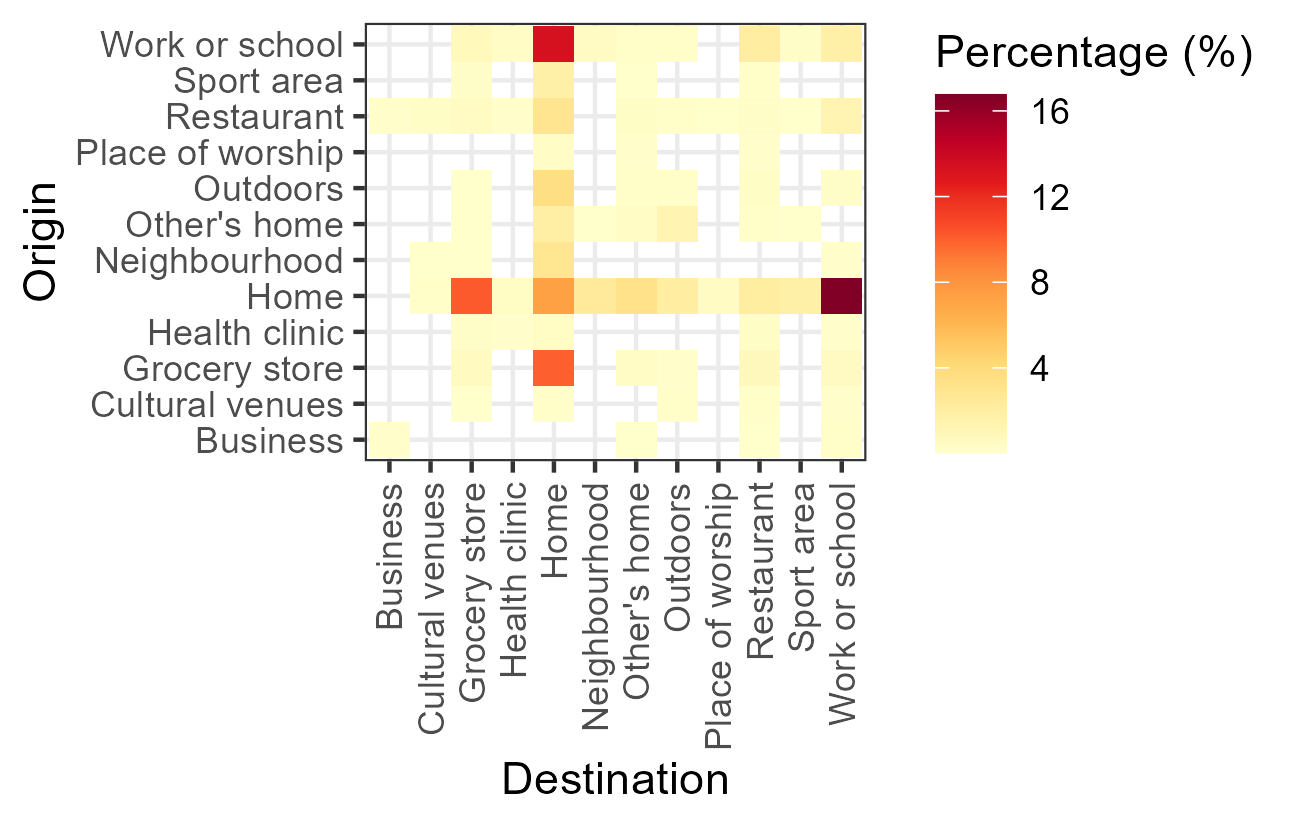
\includegraphics[width=1\linewidth]{Manuscript-figures/walking_hm_2022} 
\DIFaddendFL 

}

\caption{Percentage of walking trips categorized by origin and destination}\label{fig:figure-01}
\end{figure}

\DIFdelbegin \DIFdel{For cycling trips, Figure \ref{fig:figure-02}, shows that in 1992, when
this mode of transportation was first included as an activity, the
majority of trips were from home to work or school, accounting for about
25\% of cases. This pattern remained in 2015, with these trips
representing }\DIFdelend \DIFaddbegin \DIFadd{The \{ActiveCA\} dataset also includes information on the type of
population centre in which respondents reside - specifically, whether
they live in a CMA, a CA, or outside these areas - as well as the
respondent's province. This information is important, as patterns of
active travel often differ between metropolitan and non-metropolitan
populations. For example, Table \ref{tab:cma-durations} presents the
median walking durations by population centre type and province for
2022. Overall, respondents living in CMA/CA areas tend to report higher
median walking durations compared to those living outside these centres.
The most pronounced difference is observed in Nova Scotia: metropolitan
residents reported a median walking duration of }\DIFaddend 30 \DIFdelbegin \DIFdel{\% of
the cases. However, a notable change occurred in
home to home trips, which decreased significantly from 19\% in 1992 to }\DIFdelend \DIFaddbegin \DIFadd{minutes, whereas
non-metropolitan residents reported a median of only }\DIFaddend 5 \DIFdelbegin \DIFdel{\% in 2015.
}\DIFdelend \DIFaddbegin \DIFadd{minutes.
}\DIFaddend 

\DIFdelbegin %DIFDELCMD < \begin{figure}
%DIFDELCMD < 

%DIFDELCMD < {%%%
\DIFdelendFL \DIFaddbeginFL \begin{table}
\DIFaddendFL \centering
\DIFdelbeginFL %DIFDELCMD < 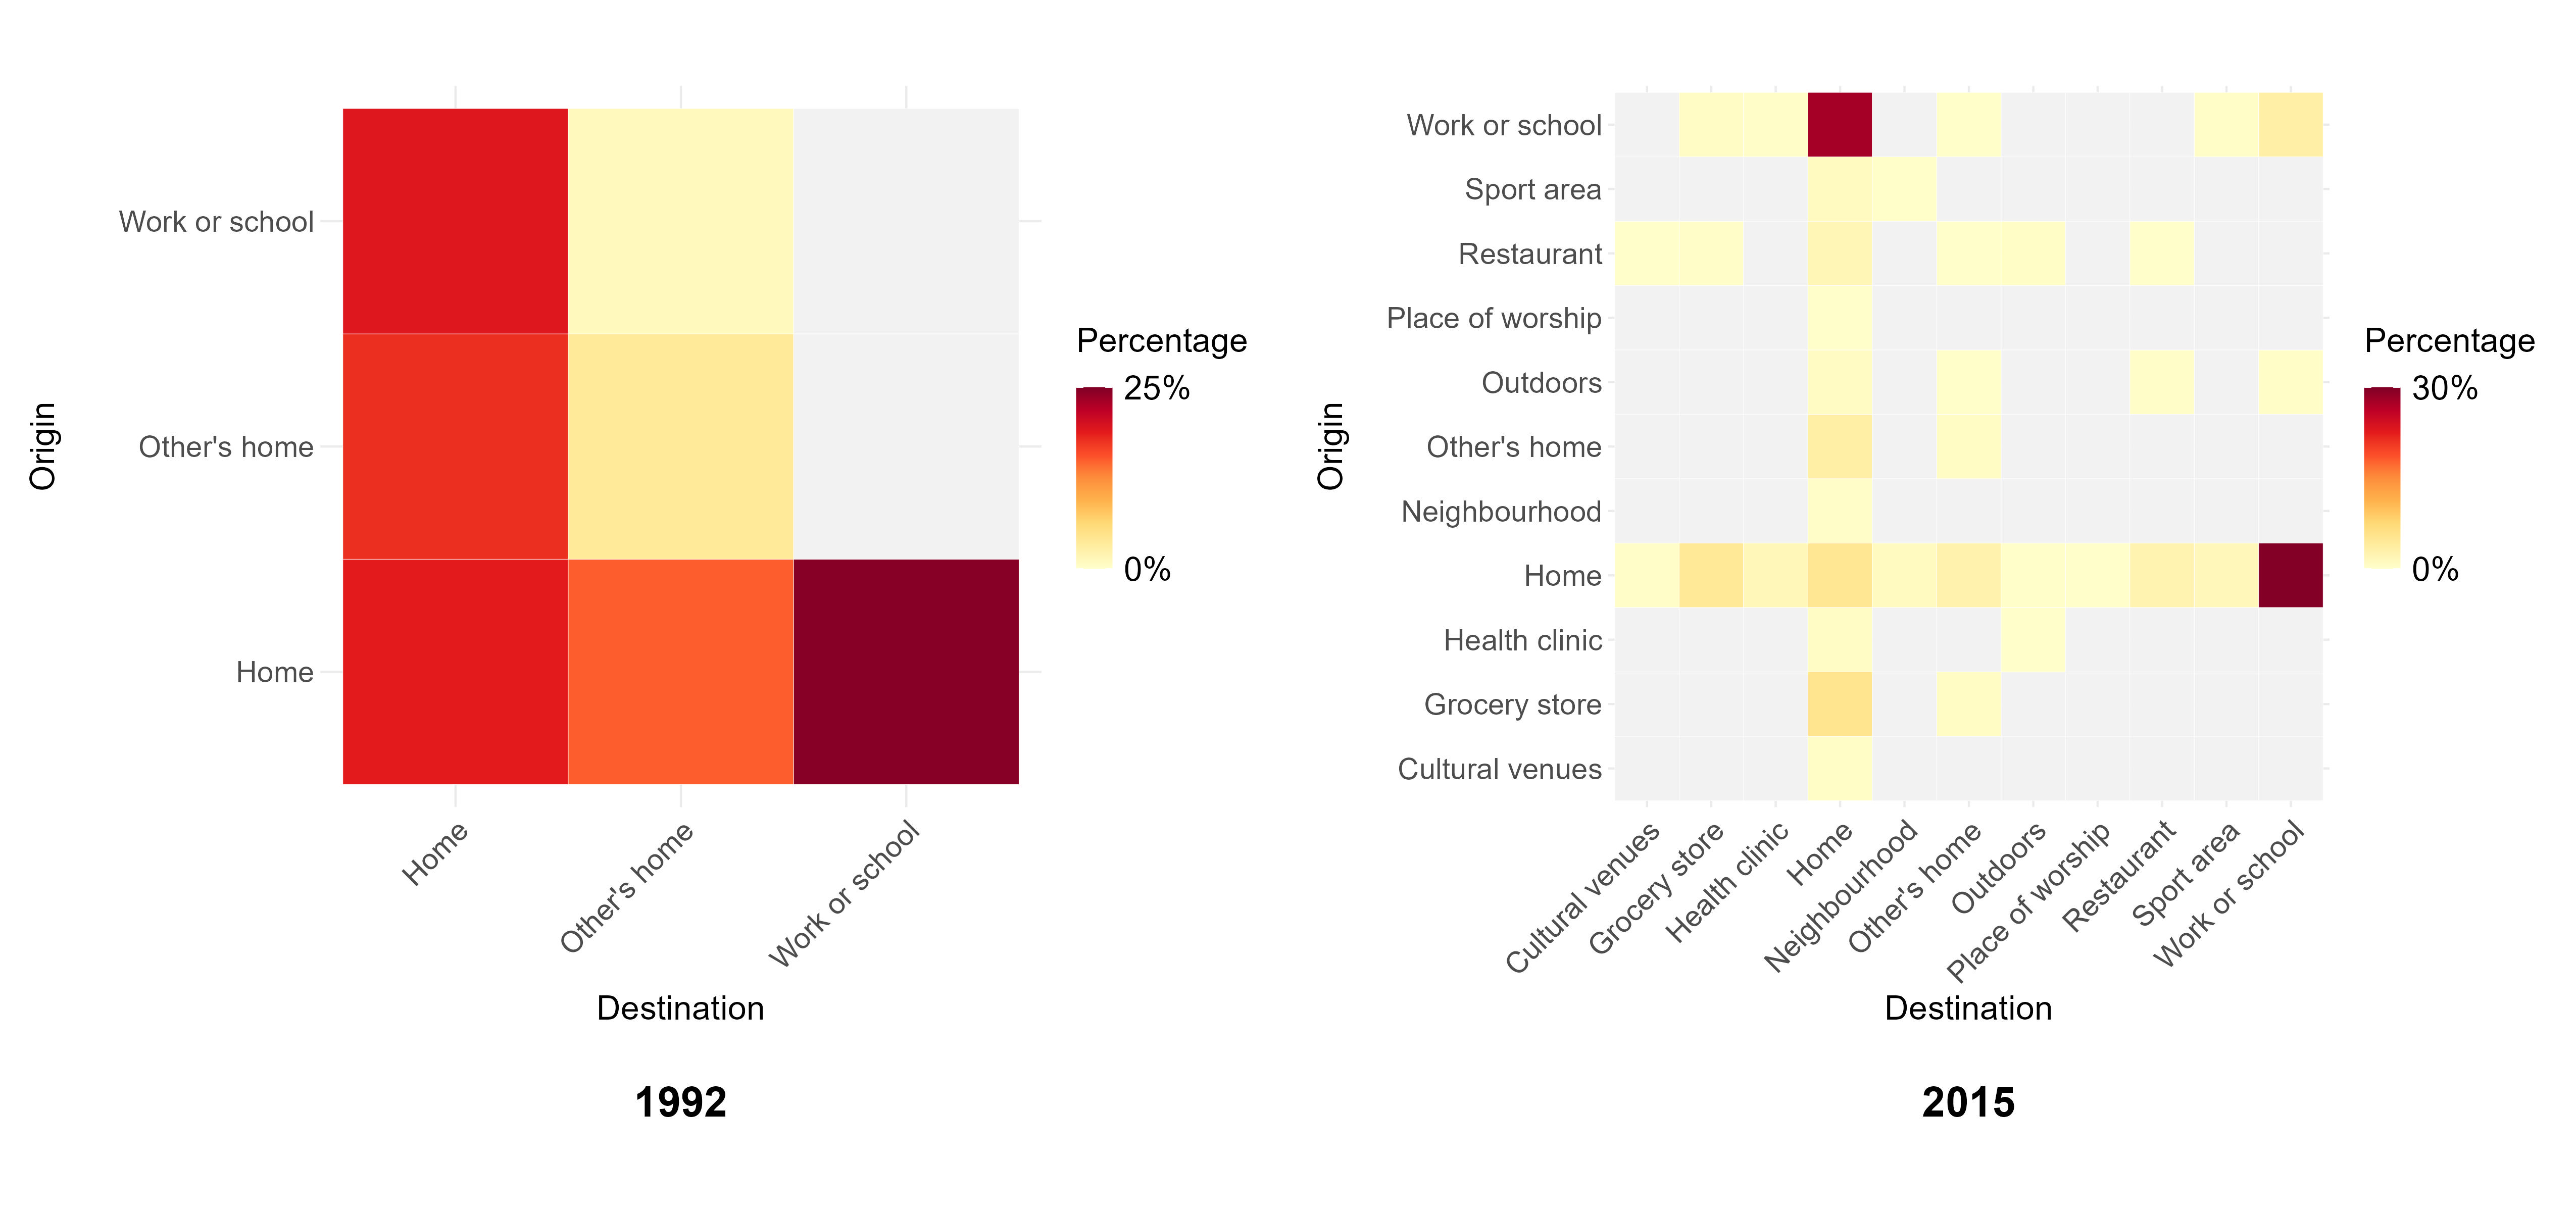
\includegraphics[width=1\linewidth]{Manuscript-figures/cycling_hm_fig} 
%DIFDELCMD < %%%
\DIFdelendFL \DIFaddbeginFL \caption{\label{tab:cma-durations}\label{tab:cma-durations}\DIFaddFL{Differences in walking duration between provinces and population centre type.}}
\centering
\resizebox{\ifdim\width>\linewidth\linewidth\else\width\fi}{!}{
\fontsize{8}{10}\selectfont
\begin{threeparttable}
\begin{tabular}[t]{lrr}
\toprule
\multicolumn{1}{c}{ } & \multicolumn{2}{c}{Population centre type} \\
\cmidrule(l{3pt}r{3pt}){2-3}
Province & CMA/CA & non CMA/CA\\
\midrule
Alberta & 15 & 5\\
British Columbia & 15 & 10\\
Manitoba & 10 & 10\\
New Brunswick & 5 & 5\\
Newfoundland and Labroador & 20 & 10\\
\addlinespace
Nova Scotia & 30 & 5\\
Ontario & 15 & 15\\
Prince Edward Island &  & 5\\
Quebec & 15 & 15\\
Saskatchewan & 10 & 5\\
\bottomrule
\end{tabular}
\begin{tablenotes}
\item \textit{Note: } 
\item CMA denotes Census Metropolitan Area and CA denotes Census agglomeration.
\end{tablenotes}
\end{threeparttable}}
\end{table}
\DIFaddendFL 

\DIFdelbeginFL %DIFDELCMD < }
%DIFDELCMD < 

%DIFDELCMD < %%%
%DIFDELCMD < \caption{%
{%DIFAUXCMD
\DIFdelFL{Percentage of cycling trips categorized by origin and destination}}%DIFAUXCMD
%DIFDELCMD < \label{fig:figure-02}
%DIFDELCMD < \end{figure}
%DIFDELCMD < 

%DIFDELCMD < %%%
\DIFdel{\{ActiveCA\} }\DIFdelend \DIFaddbegin \DIFadd{The package }\DIFaddend also enables obtaining insights from the main processed
files. Figure \ref{fig:figure-stress} present how the level of stress
varied among respondents depending on their marital status in \DIFdelbegin \DIFdel{2015.
}\DIFdelend \DIFaddbegin \DIFadd{2022.
}\DIFaddend According to this plot, married respondents reported the highest level
of stress, relating to feel stressed every day, with \DIFdelbegin \DIFdel{17}\DIFdelend \DIFaddbegin \DIFadd{15}\DIFaddend \% of possible
cases.

\begin{figure}

{\centering 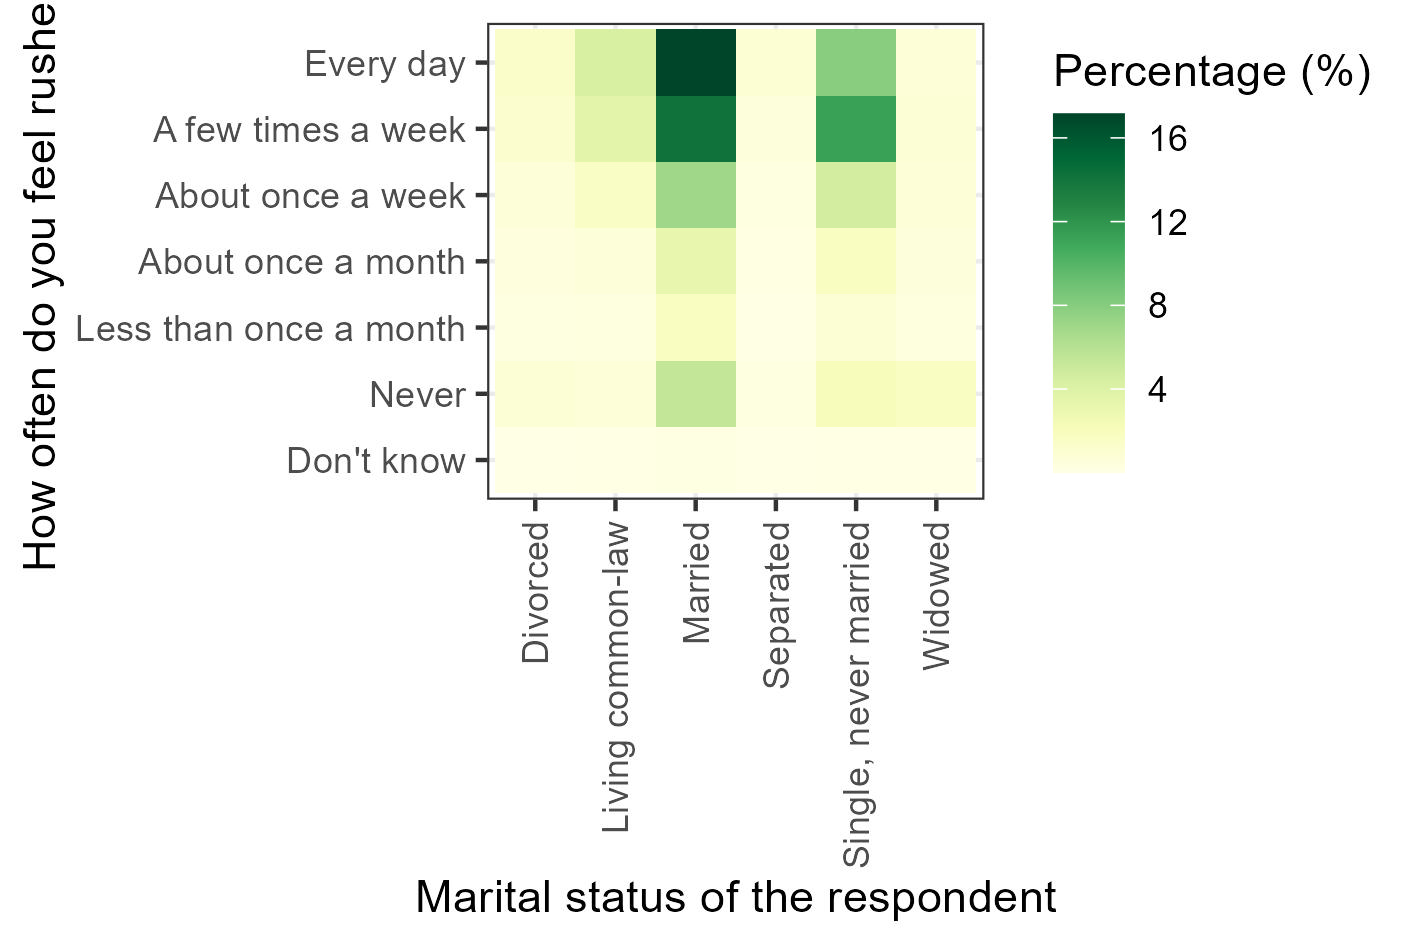
\includegraphics[width=1\linewidth]{Manuscript-figures/main_stress_figure} 

}

\caption{Level of stress among respondents of different marital statuses (2015).}\label{fig:figure-stress}
\end{figure}

\section{Python integration}\label{python-integration}

\{ActiveCA\} also provides a Jupyter Notebook containing a
\DIFdelbegin \DIFdel{Python }\DIFdelend \DIFaddbegin \texttt{\DIFadd{Python}} \DIFaddend script that demonstrates how to read \DIFdelbegin \DIFdel{R }\DIFdelend \DIFaddbegin \texttt{\DIFadd{R}} \DIFaddend data
files (.rda) and convert them into Pandas DataFrames. This process
allows users to work with and utilize the datasets available in
\{ActiveCA\} within a \DIFdelbegin \DIFdel{Python }\DIFdelend \DIFaddbegin \texttt{\DIFadd{Python}} \DIFaddend project.

\section{Concluding remarks}\label{concluding-remarks}

This paper presents \{ActiveCA\}, an open data product that provides
analysis-ready data from Cycles 2 (1986), 7 (1992), 12 (1998), 19
(2005), 24 (2010), \DIFdelbegin \DIFdel{and }\DIFdelend 29 (2015)\DIFdelbegin \DIFdel{of the GSS surveys }\DIFdelend \DIFaddbegin \DIFadd{, and 34 (2022) of TUS GSSs }\DIFaddend on active travel
in Canada. In the form of an \DIFdelbegin \DIFdel{R }\DIFdelend \DIFaddbegin \texttt{\DIFadd{R}} \DIFaddend data package, \{ActiveCA\} was
developed after collecting, cleaning, and processing the survey data,
providing information on origins, destinations, and duration of active
travel, as well other information.

\DIFdelbegin \DIFdel{It is important to remark that the present version of \{ActiveCA\}
covers all Canadian time use surveys up to 2015. While the most recent
time use survey was carried out in 2022 \mbox{%DIFAUXCMD
\citep{wray2024}}\hskip0pt%DIFAUXCMD
, the Public Use
Microdata Files are currently unavailable, and at the moment it is estimated that they will only be published in the later part of 2025.
The R package will be updated once these files become available}\DIFdelend \DIFaddbegin \DIFadd{Although we did not select non-AT episodes, the process for obtaining
them is very similar to that used for selecting AT episodes. Researchers
interested in non-AT modes can use our framework to guide their
methodology, making the small but necessary adjustments. We focused
exclusively on AT episodes because the \{ActiveCA\} package is part of a
larger project aimed at analyzing the historical evolution of active
travel behaviour in Canada}\DIFaddend .

The value of \{ActiveCA\} lies in its transparency, accessibility, and
ease of use, which facilitates the addition of complementary data sets
in the future. R users can seamlessly explore \DIFdelbegin \DIFdel{GSS }\DIFdelend \DIFaddbegin \DIFadd{TUS }\DIFaddend walking and cycling
episodes, with the option to suggest enhancements to the package as
needed. This article adopts the structure proposed by Anastasia and Páez
\citeyearpar{soukhov2023}, whose work provided essential guidance for
the creation of this package. Similarly, we aim to contribute to the
academic community by promoting transparent research practices that
encourage replication and innovation in related fields. We believe that
\{ActiveCA\} will serve as a basis for further research on \DIFdelbegin \DIFdel{GSS }\DIFdelend \DIFaddbegin \DIFadd{TUS }\DIFaddend and for
the integration of additional data by the authors or the wider open
source community.

\section{Declaration of Conflicting
Interests}\label{declaration-of-conflicting-interests}

The author(s) declared no potential conflicts of interest with respect
to the research, authorship, and/or publication of this article.

\section{Funding}\label{funding}

The author(s) disclosed receipt of the following financial support for
the research, authorship, and/or publication of this article: This work
was supported by the Social Sciences and Humanities Research Council of
Canada (\emph{More description about the funding source after the review
process}).

\section{ORCID}\label{orcid}

Author 1

Author 2

Author 3

\section{Data availability statement}\label{data-availability-statement}

The \{ActiveCA\} R data package can be found and installed on Github
(\emph{link}).

For review purposes, the package is currently available as a tar.gz file
that can be installed by R. The file can be obtained from this anonymous
location:

\url{https://user.fm/files/v2-3d261d0b2aa47fcad096cd9e49fd5cf8/ActiveCA.zip}

\bibliographystyle{sageh}
\bibliography{bibfile.bib}


\end{document}
